\documentclass[preprint,12pt,authoryear]{elsarticle}
% Neurocomputing (Elsevier) submission draft (venue per the preregistered rule B5). Build: tectonic main.tex (from unified/paper).
\usepackage{amsmath,amssymb,amsthm,booktabs,graphicx,xcolor}
\usepackage{xurl}
\usepackage[hidelinks]{hyperref}
\newtheorem{proposition}{Proposition}
\newtheorem{theorem}{Theorem}
\newcommand{\TODO}[1]{\textcolor{red}{[TODO: #1]}}
\journal{Neurocomputing}

\begin{document}
\begin{frontmatter}
\title{CapDrop: capping realized attention displacement\\ in data-limited biomedical transformers}

\author[hd]{Syeda Anshrah Gillani\corref{cor}\fnref{eq}}
\ead{syeda.gilani@stud.uni-heidelberg.de}
\author[dan,fq]{Mirza Samad Ahmed Baig\fnref{eq}}
\ead{Mirza@fandaqah.com}
\author[sz]{Shahid Munir Shah}
\author[ai]{Abdul Akbar Khan}
\author[fx]{Muhammad Omer Khan}
\author[hu]{Muhammad Hamzah Siddiqui}
\cortext[cor]{Corresponding author.}
\fntext[eq]{These authors contributed equally to this work.}
\affiliation[hd]{organization={Heidelberg University},city={Heidelberg},country={Germany}}
\affiliation[dan]{organization={Danat Fz LLC (owned by Argaam)},city={Karachi},country={Pakistan}}
\affiliation[fq]{organization={Fandaqah},city={Al Khobar},country={Saudi Arabia}}
\affiliation[sz]{organization={SZABIST University, Gharo Campus},country={Pakistan}}
\affiliation[ai]{organization={Argaam Investment},city={Riyadh},country={Saudi Arabia}}
\affiliation[fx]{organization={Fortanixor Technologies F.Z.E},country={United Arab Emirates}}
\affiliation[hu]{organization={Hamdard University},city={Karachi},country={Pakistan}}

\begin{abstract}
Attention regularizers such as attention dropout, DropKey and Relaxed Attention are set by nominal rates. A head's
output, however, is changed by the realized displacement of its attention row, $d=\tfrac12\lVert\tilde a-a\rVert_1$,
which, for targeted perturbations, depends on attention concentration. Methods compared at equal rates therefore
receive unequal doses, and no rate controls the tail of the perturbation. We derive exact expected displacements for
common attention perturbations and propose CapDrop: top-$k$ key deletion whose closed-form mixing coefficient caps
every row's displacement at a budget $\tau$. At a given mean displacement, CapDrop is the least dispersed rule in its
class. In a preregistered study, every method is calibrated to the same realized mean displacement, and the test sets
stay sealed until all 500 test-scored runs are complete. The regimes are BiomedBERT fine-tuned on 450 PubMedQA
questions per fold and a language model trained from scratch on PubMed abstracts. In the language model, CapDrop
reduced test negative log-likelihood by 0.045 nats/token versus fixed-coefficient deletion with identical deletion
draws, and by 0.032 versus tuned Relaxed Attention (multiplicity-corrected $p=0.012$; all ten seeds), contrary to our
registered expectation. A stop-gradient ablation attributes a fifth of the first gain to the gradient through the cap.
Tuned DropKey at twice the displacement remained better, by 0.058 nats/token. On PubMedQA, no attention regularizer
beat the unregularized model, and label smoothing's advantage largely vanished after temperature scaling. Matching
realized displacement exposes effects that nominal rates hide. Capping its tail improves targeted deletion, but not
beyond the strongest tuned control.
\end{abstract}

\begin{graphicalabstract}
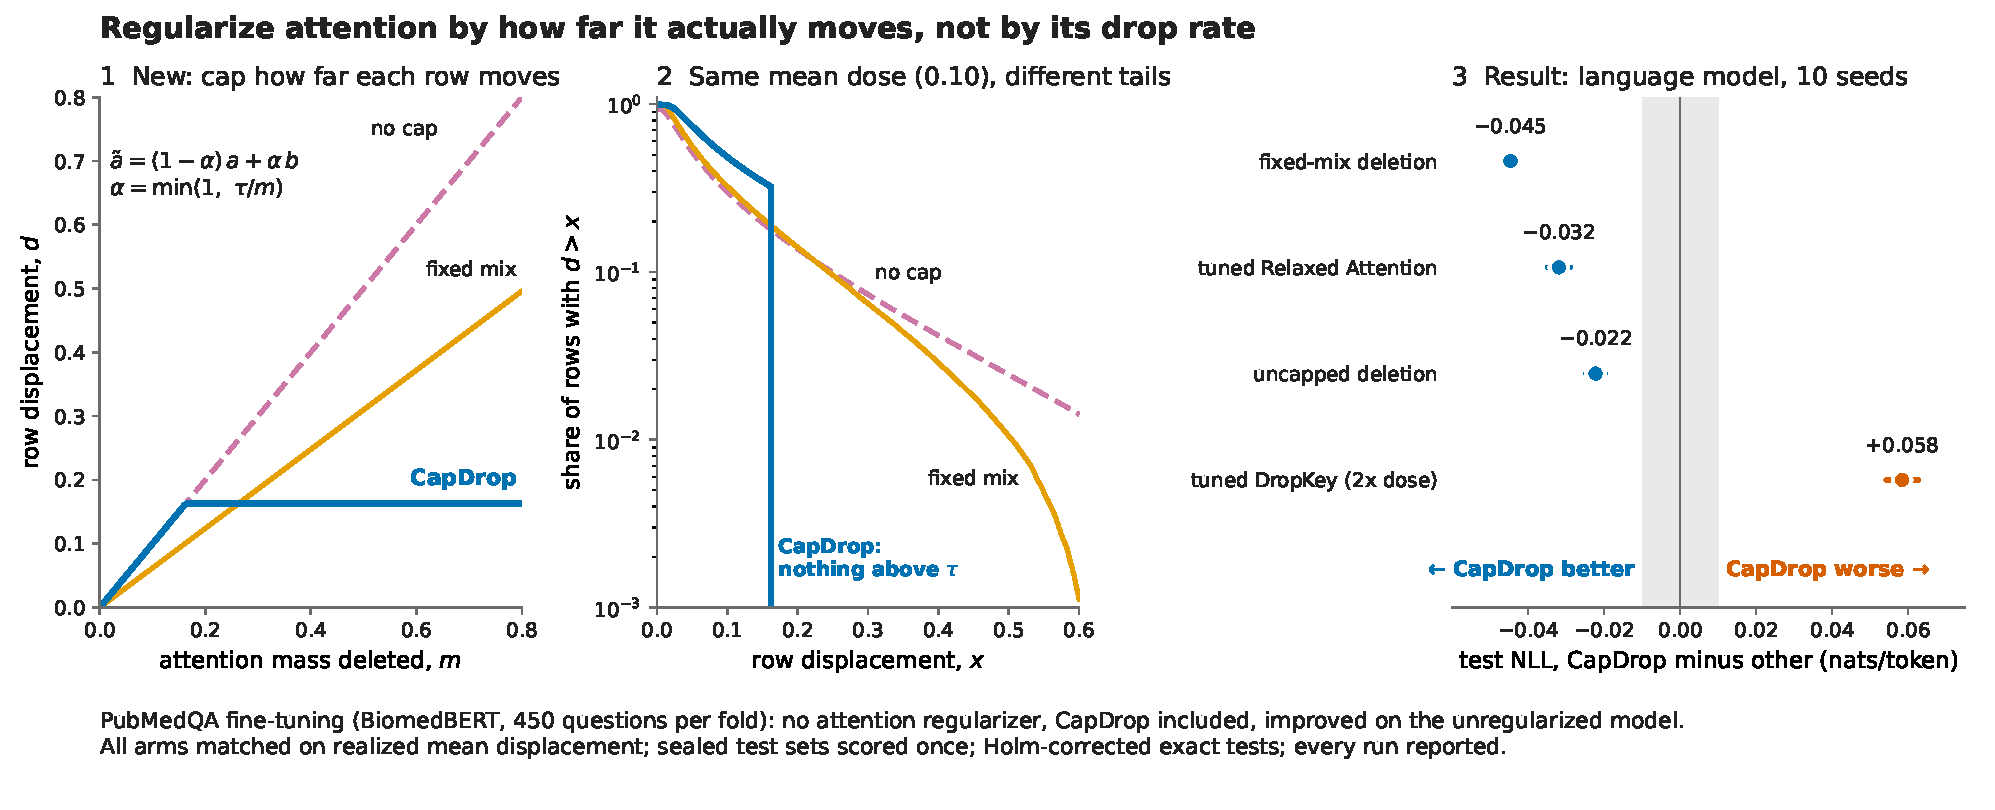
\includegraphics[width=\linewidth]{figures/graphical_abstract.pdf}
\end{graphicalabstract}

\begin{highlights}
\item CapDrop: closed-form attention deletion that caps every row's displacement
\item Preregistered comparison at matched realized displacement, not nominal rate
\item Capping the displacement tail beat fixed-mix deletion in a data-limited LM
\item Tuned DropKey at twice the displacement still beat capped deletion
\item No attention regularizer improved BiomedBERT fine-tuning on PubMedQA
\end{highlights}

\begin{keyword}
attention regularization \sep total variation \sep dropout \sep low-resource fine-tuning \sep
biomedical question answering \sep preregistration
\end{keyword}
\end{frontmatter}

% Introduction. Results-dependent sentences were written only after the single unseal, from results/analysis.json.
\section{Introduction}\label{sec:intro}

Stochastic perturbation of attention is a common regularizer for transformers
\citep{vaswani2017attention}. Attention-probability dropout, DropAttention \citep{lin2019dropattention},
DropKey \citep{li2023dropkey}, DropHead \citep{zhou2020drophead} and Relaxed Attention
\citep{lohrenz2021relaxed,lohrenz2023relaxed} are all specified by a nominal parameter: a drop rate $p$
or a mixing coefficient $\gamma$. For a single head, however, the forward pass is changed by the
\emph{realized} displacement of the attention row, $d=\tfrac12\lVert\tilde a-a\rVert_1$. If the values
have diameter $D_V$, the head output moves by at most $D_V d$ (Section~\ref{sec:theory}). How large $d$ is
for a given rate depends on how the row distributes its mass. For attention dropout the expected
displacement equals the rate. For targeted deletion it is the rate times the mass of the targeted keys.
In the pretrained BiomedBERT encoder \citep{gu2021domain}, the four highest-weighted keys hold
6.9\% of a row's mass at the 5th percentile of rows and 97\% at the 95th. The same top-4 deletion rate
therefore displaces some rows about fourteen times more than others, and on concentrated rows the displacement
is heavy-tailed.

This has two consequences. First, comparing families at equal nominal rates confounds the family with
the dose it delivers. Second, a nominal rate controls neither the mean nor the tail of the displacement.
We study a direct way to set the displacement instead. Given any candidate perturbed row $b$, the
capped mixture $\tilde a=(1-\alpha)a+\alpha b$ with $\alpha=\min\{1,\tau/\mathrm{TV}(a,b)\}$ displaces
every row by exactly $\min\{\mathrm{TV}(a,b),\tau\}$. With a top-$k$ deletion candidate we call this
CapDrop. It keeps the deletion events of the candidate and removes the part of the displacement above $\tau$.
The coefficient is radial norm clipping \citep{koloskova2023revisiting} of the displacement $b-a$ in the
total-variation (TV) norm. The operator is standard. What we add is the quantity it fixes during
training, and a test of whether fixing it matters.

That test needs a comparison at matched mean displacement, because otherwise any effect of the cap
could be an effect of a smaller dose. Among all mechanisms whose displacement lies pathwise between
zero and that of the candidate and has a given mean, truncation is minimal in convex order. This is
the classical optimality of stop-loss truncation \citep{ohlin1969class,kaas2008modern}, and it makes
CapDrop the least dispersed member of that class. A fixed-coefficient mixture of the same candidate
belongs to the same class. Comparing the two at the same realized mean displacement, with the same
deletion draws, isolates the tail of the displacement from its mean and from the candidate.

We run this comparison in two data-limited biomedical regimes where attention regularization is
plausibly relevant and fine-tuning is known to be fragile \citep{mosbach2021stability,dodge2020finetuning,zhang2021revisiting}.
The first (S1) is BiomedBERT fine-tuned on 450 expert-labelled PubMedQA questions per fold
\citep{jin2019pubmedqa}. The second (S2) is a small causal language model trained from scratch for
many epochs on a fixed PubMed corpus, a data-constrained setting \citep{muennighoff2023scaling}. Every
arm is calibrated to the same realized mean displacement, using a census of attention rows taken
before any outcome was observed. The study was preregistered with frozen code, data manifests and
analysis. Test labels and the language-model test stream were sealed and are used once, after every
declared run is complete, and every run is reported.

\paragraph{Contributions}
\begin{enumerate}
\item \textbf{Displacement accounting.} We give exact expressions for the expected realized displacement of
attention dropout, independent and top-$k$ key deletion and Relaxed Attention, together with the
second moments and the train/evaluation mean shift where these have closed forms
(Propositions~\ref{prop:deletion}--\ref{prop:laws}). We use realized displacement, rather than
nominal rate, as the axis on which families are compared. The individual identities are elementary,
and several are known.
\item \textbf{A TV cap for training-time perturbations.} For CapDrop and for TV-budgeted relaxation we
state the cap identities, the per-row output bound and the reading of $\tau$ as a dose whose
marginal effect is the measurable activation rate $\Pr(m>\tau)$ (Propositions~\ref{prop:cap}--\ref{thm:cx}).
The cap is closed form and adds $O(n)$ operations per row to the candidate.
\item \textbf{A preregistered, displacement-calibrated test.} A $2\times2$ design crosses the candidate
(uniform or deletion) with the mixing rule (fixed or capped). It is run alongside calibrated dropout,
DropKey and unbudgeted deletion, and tuned non-attention controls, in both regimes. Six confirmatory
contrasts use exact tests with Holm correction and equivalence margins, and claims follow a table of
outcomes fixed in advance. Declared extensions, run in a fixed order within a fixed compute budget,
cover a second seed, a fragile fine-tuning recipe, a second encoder, a second biomedical task,
R-Drop, budgeted DropKey, distilled students and a stop-gradient ablation of the cap. All of them completed within the budget, except a
single-epoch LM extension that did not fit.
\item \textbf{Evidence-use diagnostics and data hygiene for PubMedQA.} We evaluate every fine-tuned
model with the question only, with a label-differing mismatched abstract, and with the RESULTS
section deleted. We report these next to a question-only model trained under the same protocol. We also
document two unlabelled PubMedQA records that duplicate official test questions under different
PubMed identifiers.
\end{enumerate}

The results support a narrow claim. In the data-limited language model, CapDrop beat fixed-coefficient deletion by
0.045 nats/token at the same mean displacement and with the same deletion draws. It beat tuned Relaxed Attention by 0.032 nats/token
(both Holm-adjusted, on all ten seeds). We had registered the opposite expectation for this regime. A
stop-gradient ablation attributes about a fifth of the first difference to the gradient through the cap, and the
rest to the capped perturbation itself. The strongest tuned control, DropKey at twice the mean displacement, was better
than CapDrop by 0.058 nats/token, and we report this as a cost of the method. In PubMedQA fine-tuning, the
confirmatory contrasts were inconclusive, and no attention regularizer improved on the unregularized model. The only
significant difference, in favour of label smoothing, was a calibration effect that temperature scaling removed. The extensions did not
change this picture. Following the outcome table fixed before the study, we claim that the tail of the displacement
matters at a fixed mean in the language-model regime. We do not claim that capping is the active ingredient of
attention regularization in general.

Section~\ref{sec:related} positions the work. Section~\ref{sec:theory} develops the accounting,
and Section~\ref{sec:design} gives the preregistered design. Sections~\ref{sec:results}--\ref{sec:discussion}
report and discuss the results.

% Related work and positioning. Wording follows the verified novelty synthesis (design/novelty/synthesis.md).
\section{Related work}\label{sec:related}

\paragraph{Stochastic attention regularizers}
Several methods delete parts of the attention computation. DropAttention \citep{lin2019dropattention} and
DropKey \citep{li2023dropkey} delete attention weights or keys, and AD-DROP \citep{yang2022addrop} deletes
high-attribution positions. Scheduled DropHead \citep{zhou2020drophead} and LayerDrop \citep{fan2020reducing}
remove heads or layers. DropHead acts on head outputs rather than attention rows, so it has no row
displacement and we do not include it as an arm. Token-level masking \citep{wu2023tlm} and UniDrop
\citep{wu2021unidrop} combine several such perturbations. \citet{luo2021dropout} erase the
entries above a fraction of the row maximum and renormalize. This is the closest precedent for our top-$k$
deletion candidate.
Other methods inject noise into the attention weights: Bayesian Attention Modules \citep{fan2020bam} and
adaptive noise-augmented attention \citep{amirahmadi2025anaa}. R-Drop \citep{liang2021rdrop} regularizes
through consistency between two perturbed passes, and Mixout \citep{lee2020mixout} through mixing with the
pretrained parameters. All of these set their strength by a nominal rate, threshold or noise scale, so
the realized displacement of a row depends on how the row distributes its mass. \citet{wang2024loradropout} unify transformer dropout variants and show that DropKey and DropAttention
with normalized rescaling share a forward pass, but they compare methods at equal nominal rates.
\citet{wu2021notall} note the case in which pre-softmax masking drops every key, which needs a
fallback. Our displacement laws state such conventions explicitly, and we compare families at matched
realized total-variation (TV) distance rather than at matched nominal rate.

\paragraph{Mixing attention with a reference distribution}
Relaxed Attention \citep{lohrenz2021relaxed,lohrenz2023relaxed} mixes each row with the uniform
distribution $u$ using a constant coefficient. Its authors report that a coefficient learned per block
collapses towards zero, and they also try drawing the coefficient at random (``fuzzy relaxation'').
\citet{maekaku2022attention} extend it to learnable and previous-layer priors, with an
interpolation weight predicted per time step by a learned gate during training and inference.
\citet{utkin2022attention} form attention weights for random forests as an
$\epsilon$-contamination of the softmax. A fixed coefficient $\gamma$ bounds the displacement by $\gamma$,
but the displacement it actually produces, $\gamma\,\mathrm{TV}(a,u)$, still varies from row to row. Our TV-budgeted
relaxation fixes the displacement instead and computes the coefficient in closed form. The two rules
belong to one mixture family, and neither is a special case of the other: fixed-$\gamma$ Relaxed
Attention corresponds to the row-specific budget $\tau_{\mathrm{row}}=\gamma\,\mathrm{TV}(a,u)$.
Row-adaptive coefficients are not new in themselves. Sinkhorn normalization \citep{sander2022sinkformers} changes the
attention operator itself rather than perturbing it during training.

\paragraph{TV and mass budgets on attention}
Per-row TV budgets on attention already exist for inference-time sparsification. \citet{tzachristas2025topk} prove that the TV distance between a row and its renormalized top-$k$
truncation equals the discarded mass. They bound the output error by this distance times a value
diameter, and they choose $k$ to meet a prescribed TV budget. We use both facts and credit them.
Twilight \citep{lin2025twilight} prunes to a top-$p$ mass budget, and KV-cache eviction uses the dropped
mass as a certificate \citep{shi2026trustmass}. TV distance between attention distributions also serves as a
stability criterion for attention explanations \citep{jain2019attention,hu2023seat}. Adversarial attention
training bounds its perturbations in logit space \citep{kitada2021attention}, and the sensitivity of
softmax attention has been characterized exactly \citep{emadi2026exact} and through Lipschitz bounds
\citep{kim2021lipschitz}. Norm-based analyses show that attention weights alone do not determine a head's
effect, because the values matter \citep{kobayashi2020attention}, which is why we also measure
value-weighted displacement. Among the work we searched, none caps the realized per-row displacement of
a stochastic perturbation applied during training.

\paragraph{Clipping, trust regions and realized strength}
The coefficient $\alpha$ of Eq.~\eqref{eq:cap} is radial norm clipping \citep{koloskova2023revisiting} of the
displacement $b-a$ in the TV norm. It is not a Euclidean projection. Per-example clipping bounds each
example's contribution in differentially private training \citep{abadi2016deep}. The linearity of TV
along a mixture segment underlies conservative policy iteration \citep{kakade2002approximately}, and trust
regions and ratio clipping bound policy updates \citep{schulman2015trpo,schulman2017ppo}. Setting a perturbation by its
induced effect instead of its nominal parameter also has precedents:
\begin{itemize}
\item parameter-space noise adapted to a target distance between output distributions \citep{plappert2018parameter};
\item clipping thresholds adapted to a target unclipped fraction \citep{andrew2021adaptive};
\item DropBlock's correction of its seed rate to a realized drop rate \citep{ghiasi2018dropblock}.
\end{itemize}
Our dose identities are standard. The derivative of a limited expected value is the survival function
\citep{halliwell2012excess}, and a variable in $[0,\tau]$ has a second moment of at most $\tau$ times its mean
\citep{bartlett2005local}. The minimality of truncation in convex order is the classical optimality of
stop-loss truncation \citep{ohlin1969class,kaas2008modern}. We claim none of these as mathematical
contributions.

\paragraph{Mean versus tail of perturbations}
Classical analyses view training with small input noise as Tikhonov regularization \citep{bishop1995training} and
dropout as an adaptive quadratic penalty \citep{wager2013dropout}. Both are second-order accounts in
which the dispersion of the perturbation matters as well as its mean; Section~\ref{sec:theory} uses
the same kind of expansion as a heuristic only. Fuzzy relaxation \citep{lohrenz2023relaxed} varies the spread of
the mixing coefficient around a fixed mean in image classification and finds no significant difference
over five seeds. Bayesian Attention Modules \citep{fan2020bam} compare Weibull and lognormal attention noise
matched in mean unnormalized weight. Outside attention, truncating heavy-tailed gradient noise changes which
minima SGD reaches \citep{wang2022eliminating}. None of these matches the realized displacement or truncates
its tail. None of them tests a capped against an uncapped perturbation of the same candidate at matched mean
displacement, or repeats such a test across from-scratch language models, fine-tuned encoders and distilled
students.

\paragraph{Attention concentration}
Trained transformers put much of their attention on a few tokens: separator and special tokens
\citep{clark2019bert}, attention sinks \citep{xiao2024sinks,gu2025sinks}, high-norm artifact tokens in vision transformers
\citep{darcet2024registers} and massive activations \citep{sun2024massive}. This concentration is what makes
targeted deletion heavy-tailed. We use it only as motivation, and we measure the share of deleted mass that
falls on special tokens rather than assuming a mechanism.

\paragraph{Low-resource biomedical fine-tuning}
Fine-tuning a pretrained encoder on a small dataset is unstable across random seeds, and bias-corrected
optimization with longer training reduces this instability \citep{dodge2020finetuning,mosbach2021stability,zhang2021revisiting}.
On PubMedQA \citep{jin2019pubmedqa}, domain-specific pretraining \citep{gu2021domain,yasunaga2022linkbert} and
careful fine-tuning \citep{tinn2023finetuning} set strong encoder baselines, and compact biomedical
models are obtained by distillation \citep{hinton2015distilling,rohanian2023compact}. A teacher that sees information
unavailable to the student is an instance of learning using privileged information
\citep{vapnik2009new,lopezpaz2016unifying}. Low-rank adaptation \citep{hu2022lora} and label smoothing \citep{muller2019label}
appear here as a recipe reference point and a tuned control.

\paragraph{Evidence use on PubMedQA}
Question-only and hypothesis-only baselines expose annotation artifacts
\citep{gururangan2018annotation,poliak2018hypothesis,kaushik2018reading}. On PubMedQA the following have been reported:
question-only evaluation of the PQA-L test set for prompted LLMs \citep{lala2023paperqa,xiong2024mirage},
including section-restricted contexts \citep{sadanandan2026cot};
random-context evaluation for prompted LLMs \citep{wen2024characterizing};
a TF-IDF and linear-SVM question-only classifier trained on PQA-L, at 55.4\% accuracy \citep{huang2025selfreflective};
a fine-tuned LLM baseline without documents on an unspecified PubMedQA subset \citep{zhang2024raft};
and question-only inference on PQA-L by LLMs trained on other corpora \citep{xiao2025kailin}.
We apply question-only, label-differing mismatched-abstract and RESULTS-deletion probes to the same fine-tuned
encoders under the reasoning-required protocol, and we train a question-only reference model under that
protocol. Earlier overlap analyses match PubMed identifiers across datasets \citep{fries2022bigbio} or apply
generic $n$-gram decontamination \citep{theimerlienhard2026openmeditron}. Duplicate publication in MEDLINE is a
known phenomenon \citep{errami2008tale}, and the unlabelled PubMedQA subset has been used for training
\citep{luo2022biogpt}. We therefore report the two unlabelled records that duplicate official test questions
under different identifiers.

% Displacement accounting: definitions, exact laws, and the TV cap. Outcome-independent.
\section{Displacement accounting for attention perturbations}\label{sec:theory}

\subsection{Setting}
Fix an example, layer, head and query. Let $S$ be the set of visible keys ($n=|S|\ge 1$), let
$a$ be the softmax distribution over $S$, and let $V=(v_j)_{j\in S}$ be the value vectors, so the
head output is $z=\sum_j a_j v_j$. A training-time attention perturbation replaces $a$ by a random
row $\tilde a$ drawn by a mechanism $\mathcal M$; evaluation always uses $a$. We call
\begin{equation}
 d=\tfrac12\lVert\tilde a-a\rVert_1
\end{equation}
the \emph{realized displacement}. When $\tilde a$ is a probability vector, $d=\mathrm{TV}(a,\tilde a)$.
We summarize a mechanism on a row by its mean displacement $D=\mathbb E d$, second moment
$S_2=\mathbb E d^2$, and train/evaluation \emph{mean shift} $B=\tfrac12\lVert\mathbb E\tilde a-a\rVert_1$.
For a top-$k$ deletion candidate, $T\subseteq S$ denotes the $\min(k,n)$ keys with the largest logits,
$A_k=\sum_{j\in T}a_j$ their mass, and $a_{\max}=\max_j a_j$.

\subsection{Exact displacement laws}
\begin{proposition}[Deletion identity]\label{prop:deletion}
Let $b$ be the renormalization of $a$ after deleting a set $D\subsetneq S$ with mass $m=\sum_{j\in D}a_j<1$.
Then $\mathrm{TV}(a,b)=m$.
\end{proposition}
This identity is known from inference-time top-$k$ sparsification, where the discarded tail mass bounds the
approximation error \citep{tzachristas2025topk}; we use it for training-time perturbations.
\begin{proof}
Deleted coordinates change by $a_j$ in total $m$. Retained coordinates increase from $a_j$ to
$a_j/(1-m)$, a total increase of $\sum_{j\notin D}a_j\,m/(1-m)=m$. Half the $\ell_1$ change is $m$.
\end{proof}

\begin{proposition}[Mean displacement by family]\label{prop:laws}
With independent deletion proposals of probability $p$:
\begin{enumerate}
\item \textbf{Post-softmax attention dropout} with $\tilde a_j=a_jM_j/(1-p)$ and $M_j\sim\mathrm{Bernoulli}(1-p)$:
$D=p$ exactly and $B=0$, independently of $a$. Rows are not normalized, and
\[
S_2=\tfrac14\Bigl[\Bigl(p+\tfrac{p^2}{1-p}\Bigr)\textstyle\sum_ja_j^2+4p^2\bigl(1-\sum_ja_j^2\bigr)\Bigr].
\]
\item \textbf{Independent key deletion} (DropKey-style, all visible keys eligible, argmax restored if all
are deleted): $D=\mathbb E m=p-p^{n}a_{\max}$ and
$\mathbb E m^2=p^2+p(1-p)\sum_ja_j^2-p^{n}\bigl[1-(1-a_{\max})^2\bigr]$.
\item \textbf{Top-$k$ deletion} (same fallback): $D=\mathbb E m=pA_k-\mathbf 1\{n\le k\}\,p^{n}a_{\max}$.
\item \textbf{Relaxed Attention} ($\tilde a=(1-\gamma)a+\gamma u$, $u$ uniform on $S$): $d=\gamma\,\mathrm{TV}(a,u)$,
deterministic, so $S_2=d^2$ and $B=d$.
\end{enumerate}
\end{proposition}
\begin{proof}
(1) Coordinate $j$ contributes $a_j$ when dropped (probability $p$) and $a_jp/(1-p)$ when kept, so
$\mathbb E|\tilde a_j-a_j|=2pa_j$ and $D=p\sum_ja_j=p$; $\mathbb E\tilde a_j=a_j$. The second moment
follows by expanding $d^2=\tfrac14(\sum_ja_jc_j)^2$ with independent $c_j$, $\mathbb Ec_j=2p$ and
$\mathbb Ec_j^2=p+p^2/(1-p)$.
(2)--(3) By Proposition~\ref{prop:deletion}, $d=m$ for every realized deletion set. Linearity of
expectation gives $p\sum a_j$ over eligible keys; the fallback occurs only when all $n$ visible keys
are eligible and proposed (probability $p^n$) and restores mass $a_{\max}$. The second moment in (2)
is the variance of a Bernoulli-weighted sum plus the same fallback correction.
(4) is immediate.
\end{proof}

The individual expressions are elementary and several are known (inverted dropout is unbiased; deletion
moves the deleted mass; the all-deleted case needs an explicit convention)
\citep{srivastava2014dropout,li2023dropkey,wu2021notall,wang2024loradropout}. What is new here is using them
as a common axis on which to compare families. Proposition~\ref{prop:laws} explains why nominal rates are not comparable across families. For
dropout the rate \emph{is} the displacement; for deletion the displacement is $p$ times the mass of
the targeted keys, which varies by orders of magnitude between diffuse and concentrated heads. For
dropout and independent key deletion $D\approx p$, so the statement ``rate is not displacement'' is
specific to targeted deletion and to Relaxed Attention.

\subsection{The TV cap}
Given a candidate row $b$ with $r=\mathrm{TV}(a,b)$ and a budget $\tau\in[0,1]$, the capped mixture is
\begin{equation}\label{eq:cap}
 \tilde a=(1-\alpha)a+\alpha b,\qquad \alpha=\min\{1,\tau/r\}\ \ (\alpha=0\text{ if }r=0).
\end{equation}
With the top-$k$ deletion candidate we call this CapDrop; with $b=u$ we call it TV-budgeted relaxation (RB).
Fixed-$\gamma$ Relaxed Attention \citep{lohrenz2021relaxed,lohrenz2023relaxed} uses the same mixture with a
constant coefficient; it corresponds to the row-specific budget $\tau_{\mathrm{row}}=\gamma\,\mathrm{TV}(a,u)$, so
neither rule is a special case of the other. Input-dependent smoothing weights have been learned before
\citep{maekaku2022attention}; ours is fixed in closed form by a displacement budget and is not learned. The
coefficient $\alpha$ is radial norm clipping \citep{koloskova2023revisiting} of the displacement $b-a$ in the
TV norm: the novelty lies in the quantity it fixes during training, not in its functional form.

\begin{proposition}[Cap identities]\label{prop:cap}
For every candidate supported on $S$:
(i) $\tilde a$ is supported on $S$ and sums to one;
(ii) $\mathrm{TV}(a,\tilde a)=\min(r,\tau)$;
(iii) $\mathrm{TV}(b,\tilde a)=(r-\tau)_+$, i.e.\ the capped and uncapped perturbed rows differ by exactly the clipped excess;
(iv) for values of diameter $D_V=\max_{j,l}\lVert v_j-v_l\rVert$, $\lVert\tilde z-z\rVert\le D_V\min(r,\tau)$, and the constant is sharp;
(v) if the deletion proposals are Bernoulli$(p)$ on the $k$ eligible keys, $\Pr(m>\tau)\le 1-(1-p)^{k}$.
\end{proposition}
\begin{proof}
(i) Convex combinations of distributions on $S$ stay on $S$. (ii) By homogeneity of the norm,
$\mathrm{TV}(a,\tilde a)=\alpha r=\min(r,\tau)$. (iii) $b-\tilde a=(1-\alpha)(b-a)$, so the distance is
$(1-\alpha)r=(r-\tau)_+$. (iv) Write $w=\tilde a-a$ with positive and negative parts of equal mass
$s=\mathrm{TV}(a,\tilde a)$. Then $\sum_jw_jv_j=s(\mu_+-\mu_-)$ with $\mu_\pm$ convex combinations of the values,
whose distance is at most $D_V$ (the same bound appears for top-$k$ truncation in \citet{tzachristas2025topk}).
Moving mass $s$ between two values at distance $D_V$ attains equality.
(v) $m>0$ requires at least one proposal among $k$ keys.
\end{proof}

\begin{proposition}[Marginal dose and tail truncation; standard facts]\label{prop:dose}
For a random deleted mass $m$ with law independent of $\tau$
\citep[cf.][]{halliwell2012excess,bartlett2005local}:
(i) the right derivative of $\tau\mapsto\mathbb E\min(m,\tau)$ is $\Pr(m>\tau)$, and it is the derivative at every
continuity point of the law of $m$;
(ii) $\mathbb E\min(m,\tau)^2\le\tau\,\mathbb E\min(m,\tau)$;
(iii) $\mathbb E\min(m,\tau)+\mathbb E(m-\tau)_+=\mathbb Em$.
\end{proposition}
\begin{proof}
Part (i) follows from $\mathbb E\min(m,\tau)=\int_0^\tau\Pr(m>s)\,ds$, part (ii) from $\min(m,\tau)\le\tau$, and
part (iii) from $\min(x,\tau)+(x-\tau)_+=x$.
\end{proof}
The measured activation probability $\Pr(m>\tau)$ is therefore exactly the marginal realized dose per unit of
budget. For fixed attention rows the census (Section~\ref{sec:census}) computes it without sampling error.

\begin{proposition}[Convex-order minimality of truncation]\label{thm:cx}
Let $m\ge0$ be the deleted mass of a candidate and let $d$ be the realized displacement of any mechanism
with $0\le d\le m$ pathwise and $\mathbb Ed=\ell$. Let $\tau_\ell$ satisfy $\mathbb E\min(m,\tau_\ell)=\ell$. Then
$\min(m,\tau_\ell)\le_{\mathrm{cx}}d$: $\mathbb E\,\phi(\min(m,\tau_\ell))\le\mathbb E\,\phi(d)$ for every convex $\phi$.
In particular $S_2(\text{CapDrop})\le S_2$ of every such mechanism at the same mean displacement.
\end{proposition}
This is the classical optimality of stop-loss truncation in convex order from actuarial risk theory
\citep[Sect.~4, Theorem, via Lemma~2]{ohlin1969class}; see also \citet[Sects.~1.4 and 7.4.4]{kaas2008modern}.
Ohlin states it for retentions that are functions of the loss. The argument, reproduced below, needs only
$0\le d\le m$ and equal means, so it covers randomized mechanisms. We do not claim it as a new result; we use it to
define the matched-mean contrast between capped and uncapped perturbations.
\begin{proof}
Both variables have mean $\ell$, so convex order is equivalent to $\mathbb E(X-t)_+\le\mathbb E(Y-t)_+$ for all $t$,
with $X=\min(m,\tau_\ell)$ and $Y=d$. For $t\ge\tau_\ell$ the left side is zero. For $t<\tau_\ell$,
$\min(X,t)=\min(m,t)$, hence $\mathbb E(X-t)_+=\ell-\mathbb E\min(m,t)\le\ell-\mathbb E\min(d,t)=\mathbb E(Y-t)_+$,
using $d\le m$.
\end{proof}
The fixed-$\alpha$ mixture of the same candidate ($d=\gamma m$, arm HF) belongs to the class of
Proposition~\ref{thm:cx}; so does unbudgeted deletion at a lower rate under common random numbers
(nested deletion sets), except on rows where the all-deleted fallback applies. At matched mean
displacement the three arms therefore differ in dispersion (and in mean shift $B$), and CapDrop
is the extreme point. This is the precise sense in which the cap ``removes the tail''.

\paragraph{What the theory does not give.} The statements are exact but local: they concern one
attention row with fixed values. A second-order expansion of the loss in the head output,
$\mathbb E\ell(z+\Delta z)-\ell(z)\approx\nabla\ell^\top\mathbb E\Delta z+\tfrac12\mathbb E\Delta z^\top H\Delta z$ with
$\lVert\mathbb E\Delta z\rVert\le D_VB$ and $\mathbb E\lVert\Delta z\rVert^2\le D_V^2S_2$, motivates tracking $B$ and $S_2$ but
is a heuristic: it ignores interactions across layers and the training dynamics. Whether lower $S_2$ at matched $D$
helps or hurts generalization is an empirical question, which Section~\ref{sec:design} tests with preregistered
predictions. The gradient of \eqref{eq:cap} flows through $\alpha$; the fixed-$\alpha$ control does not have this path.

% Preregistered design (outcome-independent). Numbers in \emph{} are protocol constants.
\section{Preregistered design}\label{sec:design}

\subsection{Protocol, held-out data and integrity}
All experiments follow a protocol that was frozen, together with the code and data manifests,
before any outcome run (SHA-256 of the protocol \texttt{0b0faeb4\ldots}; the full text and every
deviation are in the supplement). The protocol fixes the arms, calibration rule, levels, seeds,
selection rules, endpoints, tests, margins and a compute budget with prespecified cut rules; it
also fixes an outcome$\to$claim table so that the headline cannot follow the results. Every declared
run is reported; no seed is replaced.

Two held-out sets are used once, after all declared runs are complete. \textbf{PubMedQA.} The official
500-question test split of the expert-labelled subset PQA-L \citep{jin2019pubmedqa} is on its second use:
it was scored once earlier in an unrelated pilot of this project with a different model family and no
selection, which we disclose. Runs score label-free test inputs in-process and write logits into
write-once sealed files; labels are read once by the unsealing script. Selection uses a seeded,
stratified 10-fold split ($450/50$) of the other 500 PQA-L questions. \textbf{Language modelling.} A fresh
test stream of 736{,}882 tokens (2{,}098 PubMed abstracts), split from the training corpus by a salted
hash of the PubMed identifier and never evaluated before. We audited every auxiliary corpus for
near-duplicates of all 1{,}000 PQA-L questions (normalized-question equality or word 5-gram Jaccard
$\ge0.5$ on the abstract). This found two records of the unlabelled PQA-U subset that duplicate
official test questions under different PubMed identifiers; they were excluded.

\subsection{Regimes}
\textbf{S1: low-resource fine-tuning.} BiomedBERT (base, abstracts and full text; 109M parameters)
\citep{gu2021domain} is fine-tuned on the 450 training questions of each fold (question and abstract as
one segment, at most 512 tokens) with a stabilized recipe for every arm: bias-corrected AdamW,
learning rate $2\times10^{-5}$, batch 16, 20 epochs, 10\% warm-up and linear decay
\citep{mosbach2021stability}, final checkpoint, no early stopping.
\textbf{S2: data-limited language modelling.} A 23.3M-parameter pre-LN causal transformer (6 layers,
width 384, context 256, byte-level BPE with 16{,}384 tokens fitted on training text) is trained from
scratch on a fixed prefix of the PubMed training stream for many epochs (Section~\ref{sec:results};
the prespecified overfitting gate and its outcome are reported there).

\subsection{Arms and displacement calibration}
Every attention arm replaces attention-probability dropout; hidden and residual dropout are fixed per
regime, so the reference arm N means ``no attention-specific regularization''. All arms share the same
materialized attention path, initialization, data order and perturbation noise stream: noise is a
counter-based function of (seed, step, layer, microbatch), which gives common random numbers across arms
and identical masks under gradient-checkpoint recomputation.

Nominal rates are not comparable across families (Proposition~\ref{prop:laws}), so each family is
\emph{calibrated} to the same realized mean displacement, $\ell=0.05$, $0.10$ or $0.20$, using the exact
expectations of Section~\ref{sec:theory}, computed on a census of eval-mode attention rows taken before
any outcome was observed: the pretrained encoder on 256 unlabelled PubMedQA inputs, and the tuned
reference LM at 10, 25, 50 and 100\% of training. The families are attention dropout (AD), DropKey-style
key deletion with its linear depth schedule (DK) \citep{li2023dropkey}, Relaxed Attention (RA)
\citep{lohrenz2023relaxed}, unbudgeted top-4 deletion (HU), and three arms that isolate the cap at the
same candidate: CapDrop (HB; $p=0.5$ unless a level requires more, $\tau$ calibrated), fixed-$\alpha$
deletion (HF; same $p$, draws and mean displacement as HB, constant $\alpha$) and TV-budgeted
relaxation (RB). Together, RA, RB, HF and HB form a $2\times2$ design
\{uniform candidate, deletion candidate\}$\times$\{fixed, capped mixing\} at $\ell=0.10$.
Tuned controls without attention perturbation complete the comparison: Mixout
\citep{lee2020mixout} and label smoothing in S1, residual dropout in S2.

\subsection{Endpoints, tests and predictions}
The primary S1 endpoint is the per-run Brier score on the official test set, with temperature-scaled
Brier (temperature fitted on each run's 50-question development fold) as a co-criterion, so that a
calibration-only effect cannot be reported as an improvement; accuracy, macro-F1 and AUROC are
secondary. The S2 endpoint is test negative log-likelihood (nats per token) at the final step and at the
best-validation step (co-primary). The confirmatory family has six contrasts, each tested with an exact
two-sided sign-flip test over ten folds (S1) or ten seeds (S2) and Holm-adjusted at $\alpha=0.05$:
H1, CapDrop versus fixed-$\alpha$ deletion at $\ell=0.10$ (the cap itself); H2, CapDrop versus the tuned
Relaxed Attention, the fixed-coefficient member of the same mixture family; H3, CapDrop versus the strongest tuned control. Null claims are
made only by equivalence (two one-sided tests; margins $\pm0.015$ Brier and $\pm0.01$ nats/token).
Directional expectations were registered from the census separation
$\delta=(S_2^{\mathrm{HF}}-S_2^{\mathrm{HB}})/\ell^2$ (Proposition~\ref{thm:cx}).

\subsection{Evidence-use diagnostics}
Every S1 model is also evaluated on the development fold and the test set with (i) the question only,
(ii) the abstract of a different question whose gold label differs (three stratified derangements,
matched on abstract length), and (iii) the RESULTS section deleted. We report the evidence-use gap
(full minus question-only accuracy), the flip rate under mismatched evidence and the rate at which
predictions follow the donor abstract's label. A question-only model trained without abstracts (Q0) and
the earlier LoRA recipe that collapsed to the majority class (L0) are reported as reference points.

\subsection{Manipulation check and audits}
Before any final run, the realized mean displacement recorded on the GPU during the tuning runs must match
across the capped and uncapped deletion arms. The ratios HB/HF and HB/HU at $\ell=0.10$ must lie in $[0.8,1.25]$;
otherwise calibration is redone once, on the average of the pretrained census and a fine-tuned census. After the core
runs, two runs per regime, chosen by a hash of the frozen protocol, are retrained twice in deterministic mode.
The two replays must agree within $10^{-6}$ and produce identical sealed files, and they must agree with the original
non-deterministic run within the between-unit standard deviation of the reference arm. Evaluation is replayed
bit-exactly from saved checkpoints.

\subsection{Preregistered extensions}
Extensions were declared with fixed run counts and a fixed order. Each one started only if its full expected cost
fitted under a hard cap of 90 GPU-hours, a rule that depends on budget and never on outcomes. Every extension that started
finished before the single unseal.
\begin{itemize}
\item \textbf{P1 (second seed).} HB and HF at $\ell=0.10$ are rerun on all ten folds with a second seed. H1-E then
uses the per-fold mean over both seeds.
\item \textbf{E2 (fragile recipe).} This extension uses the original BERT fine-tuning recipe, which is known to be unstable
on small datasets \citep{mosbach2021stability}: Adam without bias correction, three epochs, two segment embeddings. Attention dropout, CapDrop and Mixout each get 20 runs (ten folds, two seeds). A run
fails if its test accuracy is at most the majority rate (55.2\%). Failure rates are compared with attention dropout by
a one-sided permutation test stratified by fold, Holm-corrected over the two comparisons. ``No reduction'' is claimed
only if the upper 90\% bound of the reduction is below 25 percentage points. The comparison is inconclusive if
attention dropout fails in fewer than 30\% of its runs.
\item \textbf{E-S3 (distilled students).} Each fold has a teacher that also sees the abstract's conclusion. It is
never evaluated on the test set, and it must reach 65\% pooled out-of-fold accuracy on folds 0--4. A six-layer
student (layers 0, 2, \dots, 10 of BiomedBERT; 66.4M parameters) is distilled on 10{,}000 unlabelled PubMedQA questions.
It is then fine-tuned on the fold with cross-entropy plus a distillation term. The student arms are no attention
regularization, HU, HB and HF, all calibrated on a student census, plus a student trained without distillation. The
contrasts HB$-$HU and HB$-$N enter the secondary family only if the reference student reaches 57\% out-of-fold
accuracy on folds 0--4. Retention relative to the full-size model and deployment cost are reported.
\item \textbf{E5 (second encoder).} BioLinkBERT-base \citep{yasunaga2022linkbert} runs with a new census. The arms are
the reference, attention dropout at its S1-selected level, HU and HB, on the same ten folds.
\item \textbf{E4 (second task).} SciFact \citep{wadden2020scifact} uses oracle claim--abstract pairs with three labels,
trained on 919 pairs for ten epochs. The arms are the reference, the S1-selected Relaxed Attention, HU and HB, with ten
seeds. The 339 development pairs serve as a sealed one-shot test, because the official test labels are not public.
Claim-only inputs and deletion of the gold rationale sentences give the diagnostics.
\item \textbf{E1 (R-Drop).} R-Drop \citep{liang2021rdrop} is tuned on folds 0--1 over $\alpha\in\{0.1,0.5,1\}$ and compared
with CapDrop on all ten folds.
\item \textbf{E3 (targeting).} Budgeted DropKey applies the same TV cap to a candidate that deletes any key, not
only the four highest-weighted. It is calibrated to $\ell=0.10$ and compared with CapDrop in S1 and S2.
\end{itemize}
Replication in E4 and E5 is judged on HB$-$HU by the rules of H1-E. Apart from the two student contrasts, extension
contrasts are reported with unadjusted $p$-values as descriptive evidence.
Two further extensions were declared last. E6 is a single-epoch LM on an 8.0M-token prefix, a regime that does not overfit.
E8 is the CapDrop LM arm with $\alpha$ computed under stop-gradient, on ten seeds. Its forward pass and deletion
draws are identical to CapDrop's, so it isolates the gradient path through $\alpha$, which HF lacks. After E3, 85.1 GPU-hours had been used.
E6 (5.6 expected GPU-hours) did not fit under the cap and was not run. E8 (1.25 GPU-hours) fitted and was run. Its implementation, tests and
analysis rule (the H1-L rules, unadjusted, descriptive) were recorded in the freeze addendum before its first run.


\section{Results}\label{sec:results}
% Census, calibration and manipulation check. Outcome-independent: every number here comes from
% results/predictions.json (sha 16f9e895...), written before any outcome run, and from the on-device
% displacement traces of the tuning runs (studies/S1/manipulation_B11.json).
\subsection{Census, calibration and manipulation check}\label{sec:census}

\paragraph{Concentration}
The census covers 24{,}576 eval-mode rows of the pretrained encoder (2{,}048 per layer) and 49{,}152 rows of
the reference language model, pooled over four training snapshots. Encoder attention is much more
concentrated. The mean top-4 mass $A_4$ is 0.46 in the encoder and 0.21 in the LM, the median is 0.45 and 0.13,
and the mean $\mathrm{TV}(a,u)$ is 0.72 and 0.28. Across encoder rows, $A_4$ ranges from 0.069 at the 5th
percentile to 0.97 at the 95th. At $p=0.1$ and $k=4$ the dispersion index $\kappa=\mathbb E m^2/\mathbb E m$ is
0.318 in the encoder and 0.172 in the LM. The exploratory premise $\kappa_E\ge2\kappa_L$ from the protocol
therefore does not hold (0.318 versus 0.344).

\paragraph{Operating points}
Table~\ref{tab:calib} lists the calibrated parameters at $\ell=0.10$ with the exact displacement moments
implied by the census. The nominal parameters needed to reach the same mean displacement differ widely
between families. The Relaxed Attention coefficient is 0.14 in the encoder and 0.36 in the LM, and the
unbudgeted top-4 deletion rate is 0.22 and 0.49. This is Proposition~\ref{prop:laws} at work: a single nominal
rate would deliver different doses in the two regimes. Within the deletion class of
Proposition~\ref{thm:cx}, the ordering $S_2^{\mathrm{HB}}<S_2^{\mathrm{HF}}<S_2^{\mathrm{HU}}$ holds in both
regimes, as it must. CapDrop's second moment is 62\% (encoder) and 61\% (LM) of the fixed-$\alpha$ arm's. The cap binds on 54\% and 32\% of rows. The registered separation
$\delta=(S_2^{\mathrm{HF}}-S_2^{\mathrm{HB}})/\ell^2$ is 0.75 in the encoder and 0.83 in the LM. Both exceed the
prespecified threshold $c=0.5$. The registered expectations are therefore ``HB better'' for H1-E and ``HB not better
(equivalent or worse)'' for H1-L; both tests remain two-sided. An earlier protocol rule would have
registered H1-L as ``equivalent'' because the LM's median $A_4$ is below 0.2. That rule was replaced before the
freeze, and the replacement expectation includes equivalence. At $\ell=0.20$ no deletion arm reaches the level in the LM:
even at $p=1$, $\mathbb E m=0.1997$. The three deletion arms run at $p=1$ with no effective cap there, so they coincide and are run once.

Figure~\ref{fig:census} shows what the matched mean hides. At the same pooled mean of 0.10, unbudgeted and
fixed-$\alpha$ deletion leave a long tail. In the encoder, 1.3\% of HU draws displace a row by more than 0.8, and HF displacements reach 0.43.
CapDrop's displacement stops at $\tau$. Calibration pools layers, so the dose still differs between layers. Across
the encoder's layers it ranges from 0.041 to 0.151 for HU and HF, whose per-layer means coincide by construction,
and from 0.056 to 0.123 for CapDrop. The cap binds on 17\% of rows in the first layer and on 80\% in the last.

\begin{figure}[t]
\centering
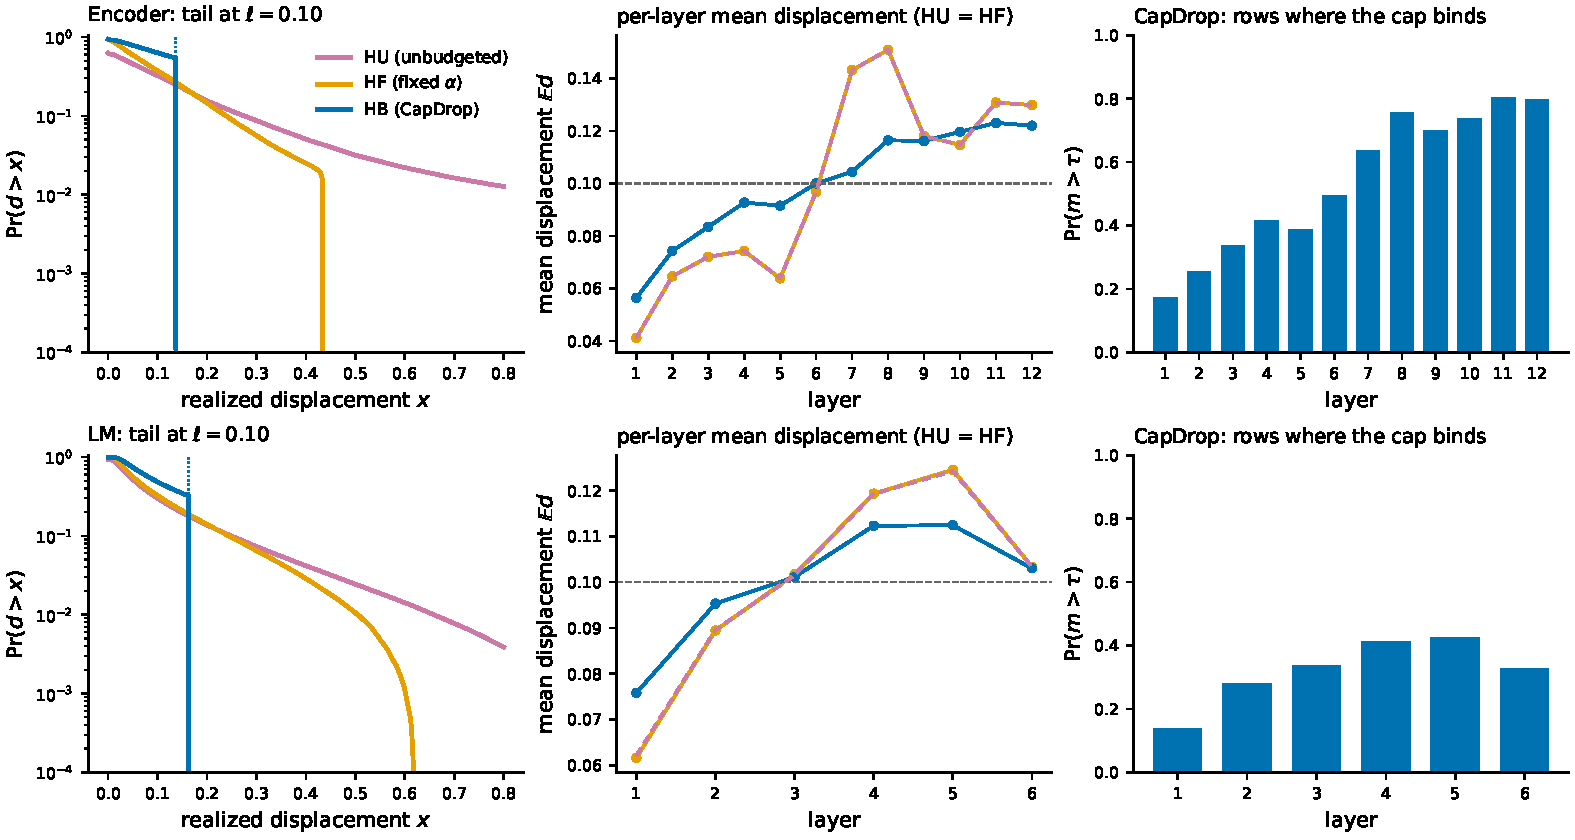
\includegraphics[width=\linewidth]{figures/fig_census.pdf}
\caption{Displacement at matched mean $\ell=0.10$ on the census rows (exact over all 16 deletion patterns of every
row; before any outcome). Left: survival function of the realized displacement $d$. Middle: mean displacement
per layer; the calibration target is the pooled mean (dashed). Right: fraction of rows on which CapDrop's cap binds.
Top: pretrained BiomedBERT; bottom: reference language model.}
\label{fig:census}
\end{figure}

\begin{table}[t]
\centering
\caption{Calibrated operating points at mean displacement $\ell=0.10$ (census, before any outcome). $S_2=\mathbb E d^2$,
$B$ is the train/evaluation mean shift and $\Pr(m>\tau)$ the fraction of rows on which the cap binds. DK uses
DropKey's linear depth schedule (maximum rate shown); its mean shift is not available in closed form.}
\label{tab:calib}
\footnotesize
\setlength{\tabcolsep}{2.6pt}
\begin{tabular}{llcccclccc}
\toprule
& & \multicolumn{4}{c}{Encoder (BiomedBERT)} & & \multicolumn{3}{c}{LM (from scratch)}\\
\cmidrule{3-6}\cmidrule{8-10}
Arm & Parameter & value & $S_2\times10^{2}$ & $B$ & $\Pr(m>\tau)$ & & value & $S_2\times10^{2}$ & $B$\\
\midrule
AD & $p$ & 0.100 & 1.25 & 0 & -- & & 0.100 & 1.08 & 0\\
DK & $p_{\max}$ & 0.185 & 2.42 & -- & -- & & 0.172 & 1.57 & --\\
RA & $\gamma$ & 0.138 & 1.09 & 0.100 & -- & & 0.361 & 1.44 & 0.100\\
RB & $\tau$ & 0.100 & 1.00 & 0.100 & -- & & 0.104 & 1.01 & 0.100\\
HU & $p$ & 0.217 & 3.59 & 0.062 & -- & & 0.491 & 2.69 & 0.079\\
HF & $p$, $\gamma$ & 0.5, 0.434 & 1.99 & 0.072 & -- & & 0.8, 0.620 & 2.12 & 0.090\\
HB & $p$, $\tau$ & 0.5, 0.137 & 1.24 & 0.070 & 0.54 & & 0.8, 0.163 & 1.29 & 0.092\\
\midrule
\multicolumn{2}{l}{$\delta=(S_2^{\mathrm{HF}}-S_2^{\mathrm{HB}})/\ell^2$} & \multicolumn{4}{c}{0.75} & & \multicolumn{3}{c}{0.83}\\
\bottomrule
\end{tabular}
\end{table}

\paragraph{Does displacement reach the head output?}
A registered value-weighted census checks whether the realized displacement of a row predicts how far the head
output moves. It is computed exactly for the top-4 deletion arms by enumerating all 16 deletion patterns, and with 64
Monte Carlo draws for AD and DK. Pooled over families at $\ell=0.10$, the Spearman correlation between $d$ and
$\lVert\Delta z\rVert$ is 0.54 in the encoder and 0.67 in the LM. Both are above the registered refutation
threshold of 0.5, so the premise of displacement accounting is not refuted, though in the encoder the margin is small.
The correlation is high for the deletion arms (0.51--0.90 in the encoder, 0.75--0.95 in the LM). It is low for
attention dropout (0.14 and 0.24), whose rows are not normalized. For TV-budgeted relaxation it is near zero,
because its displacement is almost constant. The mean relative change of the head output is 0.11--0.15 in the encoder.
The protocol also registered a secondary prediction: that the cap lowers the share of deleted mass that falls on special tokens.
This holds in the LM (1.6\% for HB versus 2.4\% for HF) but not in the encoder (16.5\% versus 14.2\%).
In the LM the value census uses the final checkpoint, whose attention is more concentrated than
the pooled calibration census. There, the arms whose displacement depends on concentration (RA and the top-4
deletion arms) have a realized mean displacement of 0.12--0.14 rather than 0.10.

\paragraph{Manipulation check}
During training, time-averaged realized mean displacement on the two S1 tuning folds was
within 6\% of its target for every calibrated arm at every level. It ranged from 0.049 to 0.051 at $\ell=0.05$, from 0.099 to 0.106
at $\ell=0.10$, and from 0.195 to 0.201 at $\ell=0.20$. The registered ratios at $\ell=0.10$ were HB/HF $=0.93$
and HB/HU $=0.97$, inside the band $[0.8,1.25]$, so no recalibration was required. We ran this check after the S1 finals had
started rather than before, which is a disclosed timing deviation; the rule's outcome
leaves the finals unchanged. Realized second moments during training matched the census
(HB 0.0121 versus 0.0124 predicted; HF 0.0233 versus 0.0199; HU 0.0385 versus 0.0359).
In the LM the check ran on the seed-1 tuning runs before the finals were declared. Time-averaged realized mean
displacement at $\ell=0.10$ was 0.111 for HB, 0.116 for HF and 0.106 for HU, giving HB/HF $=0.95$ and HB/HU $=1.05$.
Both ratios were inside the band, so no recalibration was required. The arms whose displacement depends on
concentration ran slightly above target (RA@0.10: 0.115), because LM attention concentrates during training; attention
dropout was exact. The record predates the DropKey fix described in Section~\ref{sec:discussion}. The rerun DropKey
runs realized 0.050, 0.100 and 0.200 at their three levels.

% Outcome results. Every number comes from results/analysis.json (sha 61a293a2...), written by analyze.py after the
% single unseal (results/unsealed.json, sha 149c8a73...), or from tables generated from it by tables_results.py.

\subsection{Regime checks before the finals}\label{sec:regimechecks}
\paragraph{Language-model overfitting gate}
The protocol required the language-model regime to overfit. The final validation NLL of the tuned reference model had
to end at least 0.02 nats/token above its minimum over the ten evaluations. On the first corpus (1.0M tokens, about eight
epochs) validation NLL was still falling at the last evaluation, so the gap was 0. After the single prespecified
fallback (corpus halved to 0.5M tokens, about 16 epochs over the same 977 steps), the gap was 0.008. The regime is therefore data-limited and
multi-epoch, but it overfits only mildly, and the protocol proceeds without a further fallback. The language-model
learning rate selected for the reference arm, $5\times10^{-4}$, is used by every arm.

\paragraph{Selection}
The prespecified level-selection rules chose AD@0.20, DK@0.05, RA@0.05, HU@0.05, Mixout 0.9 and label smoothing 0.2
in the encoder. They chose AD@0.20, DK@0.20, RA@0.05, HU@0.05 and residual dropout 0.2 in the LM. The strongest
tuned control was label smoothing (LS@0.2) in the encoder and DropKey (DK@0.20) in the LM. CapDrop was not tuned and
ran only at its prespecified operating point, $\ell=0.10$. This is conservative against the method: in the LM, both
tuned controls that beat it were selected at $\ell=0.20$. No top-4 deletion arm can reach that level there
(Section~\ref{sec:census}).

\subsection{Confirmatory and secondary tests}\label{sec:confirmatory}
Table~\ref{tab:confirmatory} and Figure~\ref{fig:forest} report the two families.

% Generated by tables_results.py from results/analysis.json; do not edit by hand.
\begin{table}[t]
\centering
\caption{Confirmatory family F1 (Holm over six tests) and secondary family F2. Differences are first arm minus second
arm; lower is better, so a negative difference favours the first arm. Encoder (E): test Brier, 95\% two-level bootstrap CI, co-criterion =
temperature-scaled Brier difference. LM (L): final-step test NLL (nats/token), 95\% CI by inverting the sign-flip
test, co-criterion = test NLL at the best-validation step. $p$: exact two-sided sign-flip test over ten folds or seeds
(minimum 0.002). Student contrasts S-a and S-b use test Brier.}
\label{tab:confirmatory}
\footnotesize
\setlength{\tabcolsep}{3pt}
\resizebox{\linewidth}{!}{\begin{tabular}{llcccccl}
\toprule
ID & Contrast & Diff. & 95\% CI & Co-crit. & $p$ & $p_{\mathrm{Holm}}$ & Verdict\\
\midrule
H1-E & HB@0.10 $-$ HF@0.10 & $-$0.005 & [$-$0.031, +0.009] & $-$0.003 & 0.432 & 0.863 & Inconclusive\\
H2-E & HB@0.10 $-$ RA@0.05 & $-$0.006 & [$-$0.030, +0.015] & $-$0.005 & 0.457 & 0.863 & Inconclusive\\
H3-E & HB@0.10 $-$ LS@0.2 & +0.132 & [+0.106, +0.159] & +0.009 & 0.002 & 0.012 & calibration only\\
\addlinespace
H1-L & HB@0.10 $-$ HF@0.10 & $-$0.045 & [$-$0.047, $-$0.042] & $-$0.034 & 0.002 & 0.012 & Better\\
H2-L & HB@0.10 $-$ RA@0.05 & $-$0.032 & [$-$0.035, $-$0.029] & $-$0.025 & 0.002 & 0.012 & Better\\
H3-L & HB@0.10 $-$ DK@0.20 & +0.058 & [+0.054, +0.063] & +0.056 & 0.002 & 0.012 & Worse\\
\midrule
\multicolumn{8}{l}{\emph{Secondary family F2 (separate Holm correction)}}\\
S-HBvsHU-E & HB@0.10 $-$ HU@0.10 (E) & $-$0.027 & [$-$0.054, $-$0.002] & $-$0.016 & 0.016 & 0.094 & Inconclusive\\
S-RBvsRA-E & RB@0.10 $-$ RA@0.10 (E) & $-$0.001 & [$-$0.022, +0.021] & +0.001 & 0.959 & 1.000 & Inconclusive\\
S-HBvsHU-L & HB@0.10 $-$ HU@0.10 (L) & $-$0.022 & [$-$0.025, $-$0.020] & $-$0.021 & 0.002 & 0.018 & Better\\
S-RBvsRA-L & RB@0.10 $-$ RA@0.10 (L) & +0.066 & [+0.053, +0.081] & +0.070 & 0.002 & 0.018 & Worse\\
S-a & S-HB@0.10 $-$ S-HU@0.10 & +0.016 & [$-$0.003, +0.036] & +0.011 & 0.006 & 0.041 & Inconclusive\\
S-b & S-HB@0.10 $-$ S-N & +0.000 & [$-$0.012, +0.013] & +0.001 & 0.926 & 1.000 & Equivalent\\
S-interaction-E & (HB$-$HF)$-$(RB$-$RA) (E) & $-$0.009 & -- & -- & 0.359 & 1.000 & Inconclusive\\
S-EUG & evidence-use gap, HB $-$ N & $-$0.012 & -- & -- & 0.363 & 1.000 & Inconclusive\\
S-flip & flip rate, HB $-$ N & +0.011 & -- & -- & 0.078 & 0.391 & Inconclusive\\
\bottomrule
\end{tabular}}
\end{table}


\begin{figure}[t]
\centering
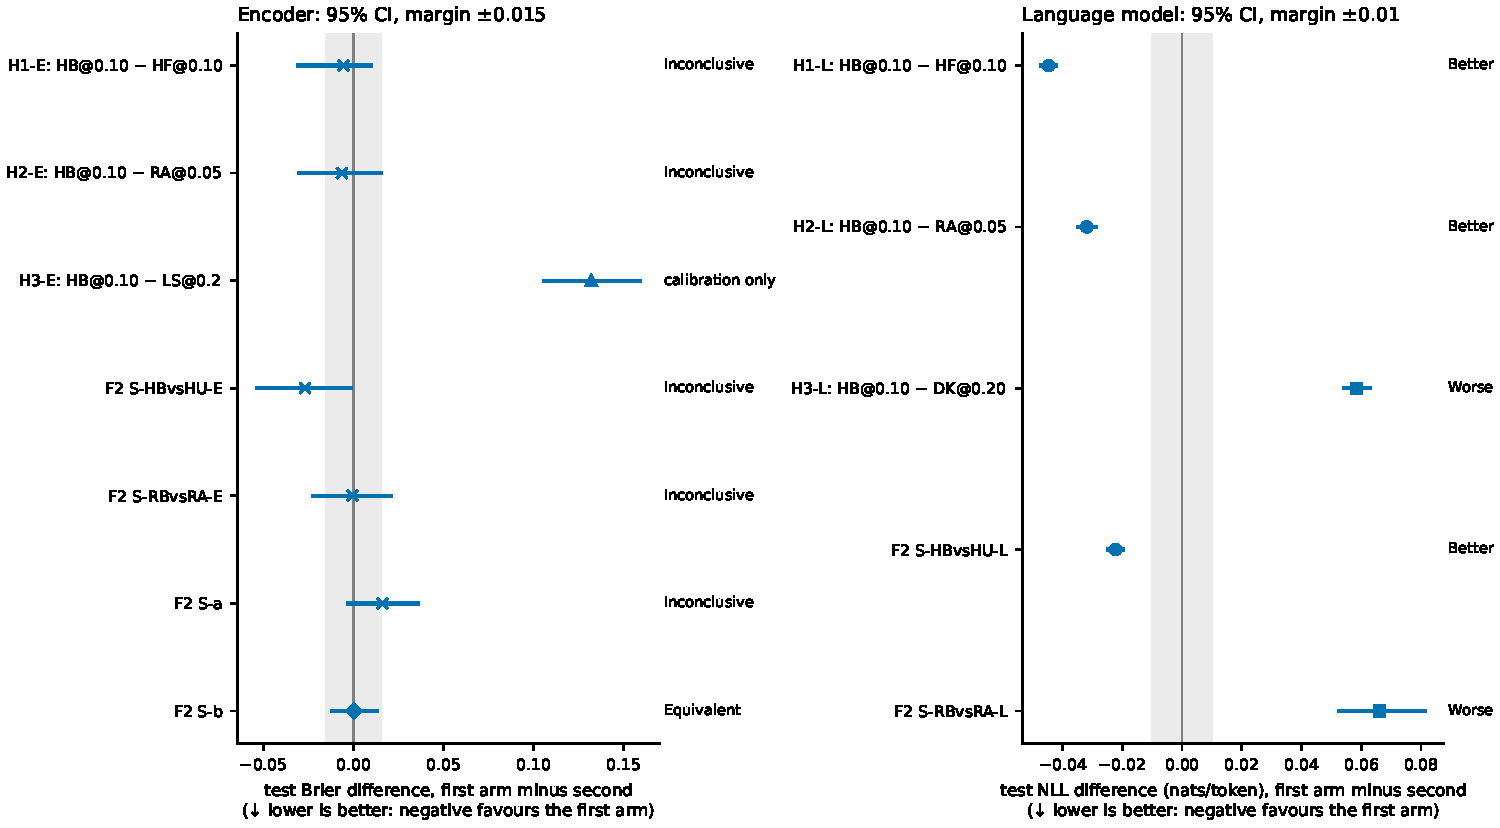
\includegraphics[width=\linewidth]{figures/fig_forest.pdf}
\caption{Confirmatory (H1--H3) and secondary (F2) contrasts with 95\% intervals and the equivalence margins (grey).
Left: encoder, test Brier. Right: language model, final-step test NLL. Verdicts follow the preregistered rules;
``calibration only'' means that raw Brier differs after Holm correction but temperature-scaled Brier does not.}
\label{fig:forest}
\end{figure}

\paragraph{Encoder (PubMedQA)}
None of the three encoder contrasts supports a claim that CapDrop is better. Against fixed-$\alpha$ deletion (H1-E), the mean
difference in test Brier was $-0.005$, with a 95\% interval of $[-0.031, 0.009]$ and Holm-adjusted $p=0.86$. Against
the tuned Relaxed Attention (H2-E), it was $-0.006$, with interval $[-0.030, 0.015]$ and Holm $p=0.86$. Both are
inconclusive. Neither a difference nor equivalence within $\pm0.015$ Brier can be claimed, because the
between-fold standard deviations of the paired differences (0.021 and 0.026) are larger than the margin allows at ten units.
Against label smoothing (H3-E), CapDrop's raw Brier was higher by 0.132 (Holm $p=0.012$). After temperature
scaling, however, the difference shrank to 0.009 and was no longer significant (raw $p=0.072$). The verdict is therefore
``calibration only''. Label smoothing produces better-calibrated probabilities (ECE 0.115 versus 0.301), and a
single temperature fitted on 50 development questions removes almost all of that advantage. Accuracy differed by
0.7 points.

\paragraph{Language model}
All three LM contrasts were decisive, and every one of the ten seeds had the same sign. CapDrop lowered final-step
test NLL relative to fixed-$\alpha$ deletion (H1-L) by 0.045 nats/token, with 95\% interval $[-0.047, -0.042]$ and Holm $p=0.012$.
The best-validation-step difference was 0.034, so the verdict is Better. This is the opposite of the registered
expectation. Because $\delta=0.83\ge0.5$, the census-based rule had registered ``HB not better'' for the LM
(Section~\ref{sec:census}). The test was two-sided, so the verdict stands, but the prediction behind it failed in the
LM. CapDrop also beat the tuned Relaxed Attention (H2-L) by 0.032 nats/token (Better). It was worse than the
strongest tuned control, DropKey at $\ell=0.20$ (H3-L), by 0.058 nats/token (Worse).

\paragraph{Secondary family}
In the LM, CapDrop beat unbudgeted top-4 deletion at the same mean displacement (S-HBvsHU-L) by 0.022 nats/token
(Holm $p=0.018$, Better). Under common random numbers, the two arms delete from the same candidate keys. In the encoder,
the same contrast favoured CapDrop by 0.027 Brier (raw $p=0.016$), but it did not survive the Holm correction
($p=0.094$, Inconclusive). TV-budgeted relaxation was worse than fixed-coefficient relaxation in the LM, by 0.066
nats/token (S-RBvsRA-L, Worse), and indistinguishable from it in the encoder. The $2\times2$ interaction in the
encoder, the evidence-use gap and the flip rate showed no effect (Holm $p\ge0.39$). In the distilled six-layer
students, the contrast S-HB$-$S-HU favoured the unbudgeted arm by 0.016 Brier. Its Holm $p$ was 0.041, but the
two-level interval included zero ($[-0.003, 0.036]$), so the verdict is Inconclusive. S-HB and the student without
attention regularization were equivalent within $\pm0.015$ Brier (S-b).

\subsection{All arms}\label{sec:allarms}
Tables~\ref{tab:arms_encoder} and \ref{tab:arms_lm} report every final arm, and Figure~\ref{fig:dose} places
them against realized displacement.

% Generated by tables_results.py from results/analysis.json; do not edit by hand.
\begin{table}[t]
\centering
\caption{PubMedQA test results by arm (BiomedBERT, ten folds; mean, with the between-fold SD of Brier in parentheses).
TS-Brier: Brier after temperature scaling fitted on each run's development fold. EUG: evidence-use gap (full minus
question-only accuracy, points). Flip: flip rate under a label-differing mismatched abstract (\%). $\bar D$: realized mean
displacement at the end of training. $\downarrow$: lower is better; $\uparrow$: higher is better. Q0 is trained on questions only and is scored here with the abstract; on its own
input format its accuracy is reported in the text. The majority-class accuracy is 55.2\%.}
\label{tab:arms_encoder}
\footnotesize
\setlength{\tabcolsep}{3pt}
\resizebox{\linewidth}{!}{\begin{tabular}{lccccccccc}
\toprule
Arm & Brier$\downarrow$ & TS-Brier$\downarrow$ & Acc.\ (\%)$\uparrow$ & Macro-F1$\uparrow$ & AUROC$\uparrow$ & ECE$\downarrow$ & EUG & Flip & $\bar D$\\
\midrule
N & 0.620 (0.022) & 0.483 & 67.0 & 0.503 & 0.718 & 0.303 & 16.0 & 58.2 & --\\
AD@0.20 & 0.638 (0.028) & 0.497 & 65.6 & 0.507 & 0.713 & 0.306 & 13.0 & 61.4 & 0.200\\
DK@0.05 & 0.632 (0.021) & 0.490 & 66.1 & 0.507 & 0.721 & 0.308 & 13.8 & 59.1 & 0.050\\
RA@0.05 & 0.626 (0.037) & 0.489 & 66.5 & 0.508 & 0.719 & 0.300 & 14.0 & 59.6 & 0.050\\
RA@0.10 & 0.635 (0.038) & 0.492 & 66.0 & 0.509 & 0.714 & 0.307 & 14.3 & 60.6 & 0.099\\
RB@0.10 & 0.634 (0.038) & 0.492 & 65.7 & 0.513 & 0.715 & 0.306 & 13.5 & 61.5 & 0.100\\
HU@0.05 & 0.629 (0.027) & 0.490 & 66.5 & 0.515 & 0.717 & 0.303 & 14.8 & 60.3 & 0.052\\
HU@0.10 & 0.647 (0.030) & 0.500 & 64.9 & 0.509 & 0.717 & 0.311 & 11.6 & 62.6 & 0.102\\
HF@0.10 & 0.630 (0.025) & 0.491 & 66.2 & 0.514 & 0.717 & 0.303 & 13.4 & 61.2 & 0.105\\
HB@0.10 & 0.620 (0.031) & 0.484 & 66.9 & 0.509 & 0.717 & 0.301 & 14.9 & 59.3 & 0.099\\
DB@0.10 & 0.630 (0.030) & 0.490 & 66.1 & 0.502 & 0.719 & 0.307 & 14.9 & 59.1 & 0.100\\
LS@0.2 & 0.488 (0.016) & 0.475 & 67.6 & 0.490 & 0.713 & 0.115 & 15.5 & 56.3 & --\\
MX@0.9 & 0.541 (0.022) & 0.485 & 66.3 & 0.472 & 0.717 & 0.201 & 15.6 & 54.9 & --\\
RDROP@0.5 & 0.632 (0.027) & 0.493 & 66.2 & 0.512 & 0.715 & 0.309 & 14.1 & 59.8 & 0.100\\
Q0 & 1.032 (0.272) & 0.725 & 30.4 & 0.228 & 0.528 & 0.447 & $-$18.9 & 36.8 & --\\
L0 & 0.574 (0.004) & 0.572 & 55.1 & 0.240 & 0.501 & 0.043 & 10.9 & 12.7 & 0.100\\
\bottomrule
\end{tabular}}
\end{table}

% Generated by tables_results.py from results/analysis.json; do not edit by hand.
\begin{table}[t]
\centering
\caption{Language-model test NLL by arm (nats/token; mean over ten seeds, between-seed SD in parentheses) at the final
step and at the best-validation step, and the corresponding perplexity ($\downarrow$: lower is better). HBsg is the extension-E8 arm (CapDrop with
$\alpha$ under stop-gradient); DB is budgeted DropKey (E3).}
\label{tab:arms_lm}
\footnotesize
\begin{tabular}{lccc}
\toprule
Arm & Final$\downarrow$ & Best-validation step$\downarrow$ & Perplexity (final)$\downarrow$\\
\midrule
N & 5.3998 (0.0027) & 5.3905 (0.0042) & 221.4\\
AD@0.20 & 5.3482 (0.0041) & 5.3480 (0.0044) & 210.2\\
DK@0.20 & 5.3161 (0.0054) & 5.3161 (0.0054) & 203.6\\
RD@0.2 & 5.4250 (0.0054) & 5.4242 (0.0059) & 227.0\\
RA@0.05 & 5.4064 (0.0029) & 5.3971 (0.0052) & 222.8\\
RA@0.10 & 5.4335 (0.0044) & 5.4211 (0.0069) & 228.9\\
RB@0.10 & 5.4996 (0.0207) & 5.4909 (0.0163) & 244.6\\
HU@0.05 & 5.3843 (0.0029) & 5.3800 (0.0040) & 218.0\\
HU@0.10 & 5.3967 (0.0036) & 5.3929 (0.0046) & 220.7\\
HF@0.10 & 5.4191 (0.0042) & 5.4057 (0.0055) & 225.7\\
HB@0.10 & 5.3745 (0.0042) & 5.3716 (0.0057) & 215.8\\
HBsg@0.10 & 5.3842 (0.0050) & 5.3819 (0.0056) & 217.9\\
DB@0.10 & 5.3779 (0.0038) & 5.3735 (0.0044) & 216.6\\
\bottomrule
\end{tabular}
\end{table}


\begin{figure}[t]
\centering
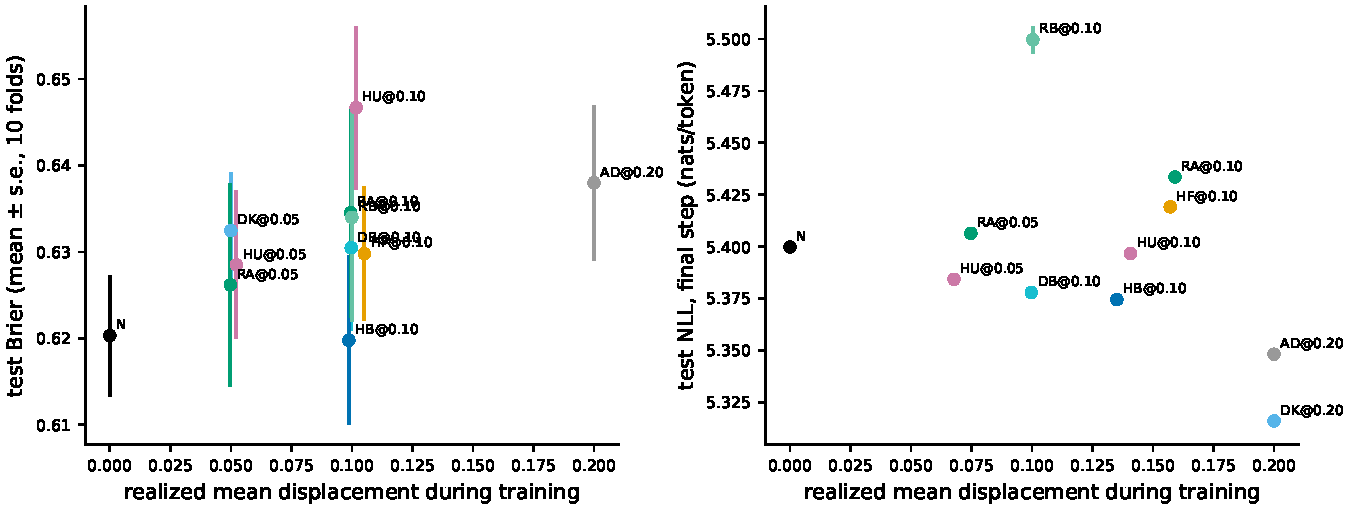
\includegraphics[width=\linewidth]{figures/fig_loss_vs_displacement.pdf}
\caption{Test loss against realized mean displacement recorded at the end of training. Left: encoder, test Brier
(mean $\pm$ s.e.\ over ten folds). Right: language model, final-step test NLL (mean over ten seeds). In the LM,
attention concentrates during training, so the realized displacement of the concentration-dependent arms (RA and
the top-4 deletion arms) at the last step exceeds the calibrated 0.10.}
\label{fig:dose}
\end{figure}

\paragraph{Encoder}
Attention regularization of any family changed little on PubMedQA. With no attention regularization, the
reference arm reached a test Brier of 0.620 and 67.0\% accuracy. Every calibrated attention arm lay between 0.620 and 0.647
Brier and between 64.9\% and 66.9\% accuracy. CapDrop matched the reference (0.620; 66.9\%), and no attention arm
improved on it. Every stabilized arm ran without failure or collapse (Figure~\ref{fig:strip}). Label smoothing and Mixout lowered
raw Brier through calibration (ECE 0.115 and 0.201, against about 0.30 for the attention arms). After temperature
scaling, all stabilized arms lay between 0.475 and 0.500. Discrimination was flat: macro AUROC ranged from 0.713 to 0.721.
The earlier LoRA recipe (L0) collapsed to the majority class in all ten folds. The question-only model (Q0) reached
49.3\% accuracy on its own question-only inputs, below the 55.2\% majority rate.

\begin{figure}[t]
\centering
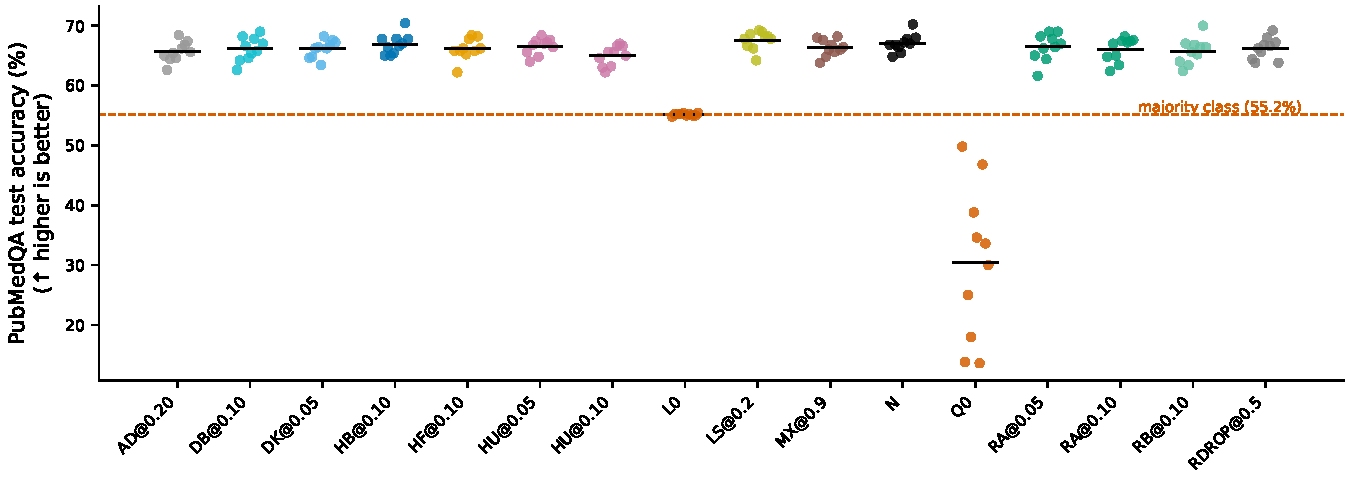
\includegraphics[width=\linewidth]{figures/fig_strip.pdf}
\caption{PubMedQA test accuracy of every run (ten folds per arm; bar: mean). Dashed: majority-class rate.
Q0 is shown on full inputs, a format it was not trained on; L0 collapses to the majority class.}
\label{fig:strip}
\end{figure}

\paragraph{Language model}
In the LM, CapDrop improved on the reference arm by 0.025 nats/token on every seed (descriptive; perplexity 215.8
versus 221.4). Fixed-$\alpha$ deletion and Relaxed Attention at $\ell=0.10$ made the reference worse, by 0.019 and
0.034. Part of the H1-L contrast is therefore harm done by HF, not only benefit from CapDrop. The two
best arms were attention dropout and DropKey at $\ell=0.20$ (5.348 and 5.316 nats/token; perplexity 203.6 for DropKey).
TV-budgeted relaxation was the worst (5.500). Validation curves (Figure~\ref{fig:lmcurves}) separate after about 500
steps and keep the same order to the end. By train-frequency bucket (descriptive), CapDrop's advantage over HF
comes from the four more frequent buckets (0.025--0.054 nats/token). On the rarest tokens it was 0.029 nats/token worse.

\begin{figure}[t]
\centering
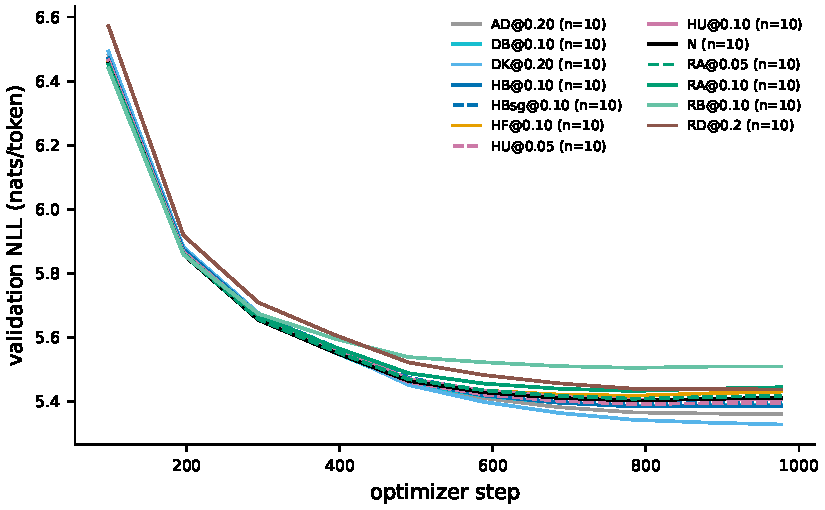
\includegraphics[width=0.8\linewidth]{figures/fig_lm_curves.pdf}
\caption{Language-model validation NLL during training, mean over ten seeds, for every arm run on all ten seeds.
Dashed: CapDrop with $\alpha$ under stop-gradient (E8) and the arms selected at $\ell=0.05$.}
\label{fig:lmcurves}
\end{figure}

\subsection{Evidence use on PubMedQA}\label{sec:evidence}
Figure~\ref{fig:evidence} shows that every fine-tuned model uses the abstract, mostly through its RESULTS section,
and that attention regularization does not change how. The evidence-use gap (full minus question-only accuracy) was
11.6--16.0 points for the stabilized arms. Their question-only accuracy (51--53\%) fell below the majority rate.
Deleting the RESULTS section lowered accuracy to 55--56\%, the majority rate. A label-differing abstract from
another question flipped 55--63\% of predictions, and about 57\% of predictions then followed the donor abstract's label.
CapDrop did not differ from the reference in evidence-use gap ($-1.2$ points) or flip rate ($+1.1$ points).

\begin{figure}[t]
\centering
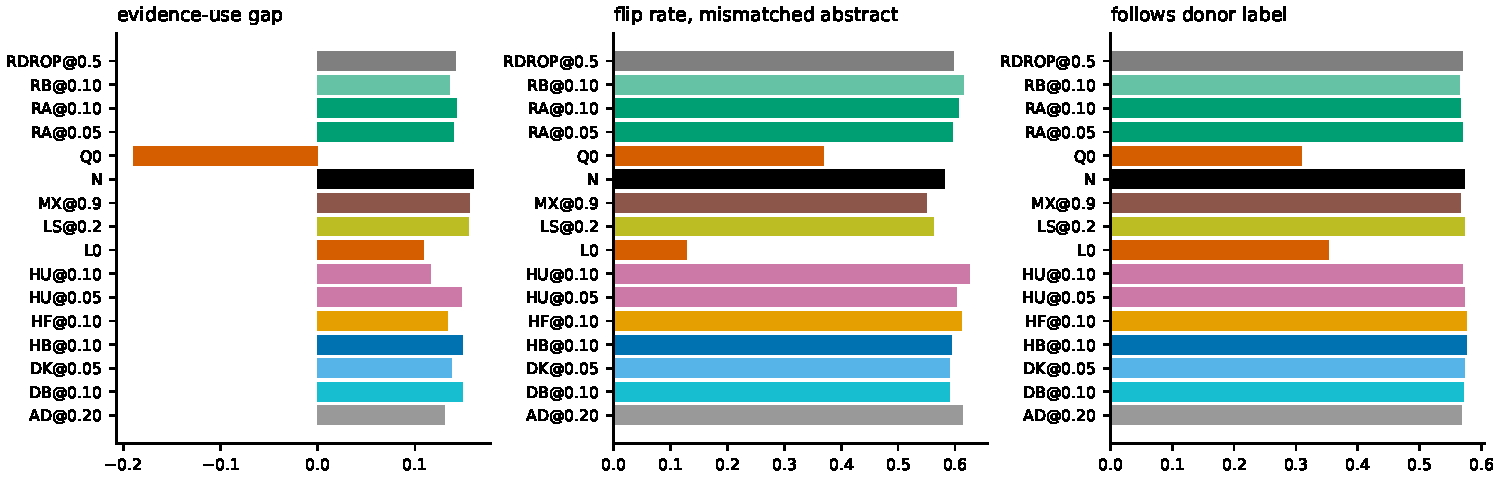
\includegraphics[width=\linewidth]{figures/fig_evidence.pdf}
\caption{PubMedQA evidence-use diagnostics on the test set (mean over ten folds). Left: evidence-use gap. Middle:
fraction of predictions that change when the abstract is replaced by one with a different gold label. Right: fraction
of predictions equal to the donor abstract's label.}
\label{fig:evidence}
\end{figure}

\subsection{Extensions}\label{sec:extresults}
Every declared extension except E6 ran to completion within the cap. Table~\ref{tab:extensions} gives the contrasts.

% Generated by tables_results.py from results/analysis.json; do not edit by hand.
\begin{table}[t]
\centering
\caption{Extension contrasts (descriptive; unadjusted $p$, verdicts by the H1 rules). Encoder rows: test Brier (E4:
SciFact development set used once as a test), 95\% two-level bootstrap CI, co-criterion = TS-Brier difference.
LM rows: final-step test NLL; $^\dagger$90\% paired-$t$ interval used for equivalence (margin $\pm0.010$);
co-criterion = best-validation-step difference. Differences are first arm minus second arm; lower is better, so a
negative difference favours the first arm. E2 (failure rates) is reported in the text; E6 was not run (budget).}
\label{tab:extensions}
\footnotesize
\setlength{\tabcolsep}{3pt}
\resizebox{\linewidth}{!}{\begin{tabular}{lllcccl}
\toprule
Extension & Contrast & Diff. & CI & Co-crit. & $p$ & Verdict\\
\midrule
P1 (seed 2) & HB@0.10 $-$ HF@0.10 & $-$0.001 & [$-$0.024, +0.021] & +0.000 & 0.916 & Inconclusive\\
B6 OOF, H2-E & HB@0.10 $-$ RA@0.05 & +0.004 & [$-$0.017, +0.025] & +0.001 & 0.562 & Inconclusive\\
B6 OOF, H3-E & HB@0.10 $-$ LS@0.2 & +0.131 & [+0.103, +0.160] & +0.008 & 0.008 & calibration only\\
E-S3 & S-HB@0.10 $-$ S-HF@0.10 & +0.010 & [$-$0.004, +0.026] & +0.007 & 0.061 & Inconclusive\\
E-S3 & S-N $-$ S-noKD & +0.014 & [$-$0.038, +0.065] & +0.010 & 0.031 & Inconclusive\\
E5 BioLinkBERT & HB@0.10 $-$ HU@0.10 & +0.001 & [$-$0.021, +0.023] & $-$0.000 & 0.930 & Inconclusive\\
E5 BioLinkBERT & HB@0.10 $-$ N & +0.006 & [$-$0.013, +0.027] & +0.005 & 0.305 & Inconclusive\\
E5 BioLinkBERT & HU@0.10 $-$ N & +0.006 & [$-$0.017, +0.030] & +0.005 & 0.492 & Inconclusive\\
E5 BioLinkBERT & AD@0.20 $-$ N & $-$0.001 & [$-$0.026, +0.025] & +0.000 & 0.951 & Inconclusive\\
E4 SciFact & HB@0.10 $-$ HU@0.10 & +0.028 & [+0.005, +0.051] & +0.007 & 0.020 & calibration only\\
E4 SciFact & HB@0.10 $-$ N & +0.022 & [$-$0.005, +0.052] & +0.026 & 0.045 & Inconclusive\\
E4 SciFact & HU@0.10 $-$ N & $-$0.007 & [$-$0.040, +0.028] & +0.019 & 0.609 & Inconclusive\\
E4 SciFact & RA@0.05 $-$ N & +0.019 & [+0.001, +0.037] & +0.018 & 0.004 & Worse\\
E1 R-Drop & HB@0.10 $-$ RDROP@0.5 & $-$0.013 & [$-$0.040, +0.014] & $-$0.009 & 0.287 & Inconclusive\\
E3 (encoder) & DB@0.10 $-$ HB@0.10 & +0.011 & [$-$0.012, +0.035] & +0.006 & 0.295 & Inconclusive\\
E3 (LM) & DB@0.10 $-$ HB@0.10 & +0.003 & [+0.002, +0.005]$^\dagger$ & +0.002 & 0.012 & Equivalent\\
E8 (LM) & HBsg@0.10 $-$ HB@0.10 & +0.010 & [+0.008, +0.011]$^\dagger$ & +0.010 & 0.002 & Worse\\
\bottomrule
\end{tabular}}
\end{table}


\paragraph{Second seed, out-of-fold replication and second encoder}
The second seed (P1) gave the same H1-E picture, with a difference of $-0.001$ Brier. The out-of-fold replication of the
encoder selection on folds 2--9 reproduced the H2-E and H3-E verdicts. With BioLinkBERT (E5), no contrast differed from zero,
and HB$-$HU was $+0.001$.

\paragraph{Second task (E4, SciFact)}
On SciFact, CapDrop's raw Brier was higher than unbudgeted deletion's by 0.028. The difference vanished after temperature
scaling ($+0.007$), so this too is calibration only, with the opposite sign to the PubMedQA encoder.
Relaxed Attention was worse than the reference by 0.019 Brier on both criteria. Under the replication rule, neither E4 nor E5
reproduces the H1-E verdict.

\paragraph{Fragile recipe (E2)}
Under the original BERT recipe, attention dropout failed (test accuracy at most the majority rate) in 19 of 20 runs.
CapDrop and Mixout each failed in 15 of 20. The reduction of 20 points was not significant for either arm
(Holm $p=0.22$; 90\% intervals $[0, 40]$ and $[5, 40]$ points). The upper bounds exceed 25 points, so ``no reduction''
cannot be claimed either. The comparison is inconclusive.

\paragraph{Distilled students (E-S3)}
The privileged teachers passed their gate (70.8\% pooled out-of-fold accuracy on folds 0--4). The reference
student passed its gate too (58.8\%), so S-a and S-b entered the secondary family (above). Students kept 91.2--92.8\% of the
full model's PubMedQA accuracy with 61\% of its parameters. At 384 tokens they halve batch-1 latency on the GPU
(5.9 versus 11.1\,ms) and on four CPU threads (112 versus 226\,ms), and double GPU throughput (326 versus 166 sequences/s).
Distillation itself did not measurably change Brier (S-N$-$S-noKD: $+0.014$, interval $[-0.038, 0.065]$).

\paragraph{R-Drop (E1) and targeting (E3)}
R-Drop with the selected $\alpha=0.5$ did not differ from CapDrop ($-0.013$ Brier, $p=0.29$) and took 2.4 times
as long to train. Budgeted DropKey, which applies the same cap to a candidate that may delete any key, was
indistinguishable from CapDrop in the encoder. In the LM it was equivalent within $\pm0.010$ nats/token
($+0.003$; 90\% interval $[0.002, 0.005]$).

\paragraph{Gradient path (E8)}
CapDrop's gradient flows through $\alpha=\min(1,\tau/m)$, and fixed-$\alpha$ deletion has no such path. E8 removes the path
by computing $\alpha$ under stop-gradient, which leaves the forward pass and every deletion draw unchanged. This raised test NLL by
0.0097 nats/token on every seed (90\% interval $[0.008, 0.011]$; best-validation step 0.010; descriptive). The
detached variant still beat fixed-$\alpha$ deletion by 0.035 and unbudgeted deletion by 0.013 nats/token, again on every
seed (descriptive, paired by seed). About four fifths of the H1-L difference therefore comes with the capped forward
perturbation itself, and about one fifth with the gradient through $\alpha$.

\paragraph{E6}
The single-epoch LM extension (E6) was not run. After E3, 85.1 GPU-hours had been used, and E6's expected 5.6 GPU-hours
would have exceeded the 90-hour cap. E8 (1.25 GPU-hours) fitted under the cap and was run.

\subsection{Audits, exploratory analyses and compute}\label{sec:audits}
Two runs per regime, chosen by a hash of the protocol, were retrained twice in deterministic mode. Each pair agreed exactly
(maximum difference 0) and produced identical sealed files. The original non-deterministic runs agreed with the
replays within the registered tolerance (largest deviation 0.010 dev Brier against a tolerance of 0.137). Evaluation
replays from saved checkpoints were bit-identical.

Exploratory analyses were as follows. The encoder dose--response over matched pairs was flat (Spearman $\rho=-0.24$, $p=0.71$, six
points). Brown--Forsythe tests found no difference in between-fold variance between CapDrop and HF, HU, RA or N ($p\ge0.28$). The descriptive
displacement-accounting model (per-run test Brier on realized $\bar D$, realized $S_2$, census $B$ and fold effects,
fitted on N, AD, DK and RA) had $R^2=0.85$ including fold effects. It predicted the HU, HF, HB and RB arms within
0.012 Brier. It is not a mediation analysis.

The campaign used 86.3 GPU-hours of compute (thermal pauses excluded) on one 4\,GB laptop GPU, within the 90-hour
cap. Every declared run completed and none was cut. The only replaced runs are the three DropKey LM tuning runs
that were excluded before any test outcome was seen (Section~
ef{sec:discussion}).


% Discussion. The limitations are fixed by the design and the protocol's claim boundaries; the
% interpretation of outcomes is written only after the unseal.
\section{Discussion}\label{sec:discussion}

\paragraph{What the results support}
The preregistered outcome table maps these verdicts to one claim. H1 is Better in one regime (the LM), and H3 is not Better in either
regime (Worse in the LM, calibration only in the encoder). The supported claim is therefore restricted:
\emph{at a fixed mean, the tail of the attention displacement matters in the data-limited language model}. Capping
the tail of top-4 deletion beat fixed-coefficient deletion with the same deletion draws, unbudgeted deletion
from the same candidate keys, and the tuned Relaxed Attention. It also beat no attention regularization. Capping did
not beat the strongest tuned control, and the protocol requires that this result be reported as a cost of the method. We make no claim that tail
capping is the active ingredient of attention regularization in general. We also make no claim for PubMedQA fine-tuning,
where the confirmatory contrasts were inconclusive and no attention family improved on the unregularized reference.

\paragraph{The registered LM expectation failed}
From the census separation, we had registered that CapDrop would \emph{not} beat fixed-$\alpha$ deletion in the LM.
The reasoning was that in an overfitting regime the second-order term $\mathbb E d^2$ regularizes, and the cap minimizes it.
The opposite happened, and by a wide margin. Two observations bear on why, though neither was a registered test. First, the regime overfitted
only mildly: it failed its overfitting gate even after the fallback. Second, in this regime the heavy-tailed arms at
$\ell=0.10$ \emph{hurt}. Fixed-$\alpha$ deletion and Relaxed Attention were worse than no attention regularization, and
unbudgeted deletion was about neutral. Removing the tail turned a harmful perturbation into a helpful one. A
convex-order argument tells us which arm has the least dispersed displacement, but not whether dispersion helps or harms.
These results show that the sign is regime-dependent, and that a census statistic alone did not predict it.

\paragraph{The cap is not uniformly beneficial}
TV-budgeted relaxation, the cap applied to a uniform candidate, was clearly worse than Relaxed Attention in the LM.
With $\tau=0.10$ below almost every row's distance to uniform, it displaces nearly every row by the same amount, so
diffuse rows are perturbed as much as concentrated ones. The benefit we observe is specific to capping a heavy-tailed
deletion candidate. Capping as such did not help. The targeting extension agrees with this. Applied to a candidate that may delete
any key, the same cap was equivalent to CapDrop in the LM.

\paragraph{Gradient path}
CapDrop and fixed-$\alpha$ deletion differ in their gradients as well as in their forward perturbation. The stop-gradient ablation
(E8) separates the two. Removing the gradient through $\alpha$ cost about 0.010 nats/token. The detached arm still beat fixed-$\alpha$
deletion by 0.035, so most of the H1-L difference comes with the capped forward perturbation. The ablation is descriptive and
is not part of the confirmatory family.

\paragraph{DropKey and dose}
DropKey and attention dropout, both selected at $\ell=0.20$, gave the lowest LM test loss. CapDrop was fixed by
design at $\ell=0.10$, and in the LM no top-4 deletion arm can deliver 0.20, because even $p=1$ removes only 0.1997
of the mass on average. H3-L therefore compares CapDrop at its prespecified dose with a competitor at twice the
dose. The design cannot say whether the difference is one of form or of dose. Our data are consistent with dose: the two best arms were also the two highest-dose arms, and attention
dropout, the least targeted family, beat every arm at $\ell=0.10$. A capped candidate
that can reach larger displacements, such as budgeted DropKey at a higher $\tau$, is the natural next test. It was not part of
this protocol.

\paragraph{Fine-tuning on PubMedQA}
On 450 training questions per fold, the between-fold variability of the paired Brier differences (SD 0.02--0.03) was
larger than every attention effect. All calibrated attention arms lay within 0.027 Brier of the reference, and the
second encoder, the second task and the fragile recipe showed no consistent advantage either. Any benefit of attention
regularization in this regime is smaller than our design could detect (about one between-fold SD at ten units). The
difference that did reach significance came from label smoothing, and it was calibration: a single temperature fitted on 50 development
questions removed it. For practitioners in this regime, temperature scaling is cheaper than any regularizer we tested.

\paragraph{How the fine-tuned models use evidence}
Every stabilized model used the abstract, mainly its RESULTS section. Deleting RESULTS lowered accuracy to the majority rate, and question-only
evaluation fell below it. A label-differing abstract changed about 60\% of the predictions. Neither the question-only
model trained under the same protocol (49.3\%) nor the question-only evaluation of the fine-tuned models
reached the majority rate. In this setting, PubMedQA accuracy reflects reading the abstract rather than question
priors. To our knowledge, and in the literature we searched, these are the first fine-tuned question-only and
mismatched-evidence baselines reported on PQA-L.

\subsection{Limitations}
\paragraph{Scope}
All models have at most 110M parameters and were trained on English biomedical text with one 4\,GB laptop GPU, using
non-deterministic bf16 kernels. The confirmatory statements hold at the prespecified operating points: top-4
deletion, a mean displacement of 0.10 and the calibrated proposal rate. We make no state-of-the-art claim,
because larger biomedical encoders report higher PubMedQA accuracy \citep{yasunaga2022linkbert,tinn2023finetuning}, and no clinical claim.

\paragraph{Held-out data}
The official PubMedQA test set is on its second use: it was scored once in an unrelated earlier pilot, with no
selection. Inference about it is therefore conditional on that set. The language-model test stream and the SciFact
evaluation set had not been evaluated before in this project. With ten units per contrast, the exact sign-flip test has a minimum two-sided $p$ of
0.002. The detectable effect is about one to 1.3 between-unit standard deviations at 80\% power. ``Inconclusive'' is a
possible and legitimate verdict.

\paragraph{What the matched-mean test isolates}
CapDrop and fixed-$\alpha$ deletion share the candidate, the deletion draws and the mean displacement, but they
differ in more than the tail. Their mean shifts $B$ differ slightly (Table~\ref{tab:calib}). The rows on which the cap
binds are the concentrated ones. Only CapDrop's gradient flows through $\alpha$; in the LM, the stop-gradient ablation (E8) separates this part. We state this bundle as the
contrast, rather than claiming to isolate the tail alone. Calibration pools rows over layers, so per-layer doses
differ between arms (Figure~\ref{fig:census}). The theory is local to one row with fixed values; the second-order
reading is a heuristic, and the descriptive displacement-accounting model is not a mediation analysis.

\paragraph{Deviations}
The language-model regime did not meet its prespecified overfitting criterion, even after the single
allowed fallback. The regime is multi-epoch and data-limited, but it overfits less than planned. The manipulation check was
run after the encoder finals had started; it required no recalibration. The language-model runner initially ignored
DropKey's depth schedule. The manipulation record revealed this before any test outcome was seen: the three affected
tuning runs had about 1.7 times their calibrated displacement. They were excluded, unopened and reported, and rerun
after the fix, and the unchanged selection rule was applied again. The TV-budgeted relaxation and budgeted-DropKey
language models do not fit in the free GPU memory, so they use activation checkpointing, which gave bit-identical
losses and gradients in a probe. The audit replays were implemented after the freeze and before the unseal. The protocol capped the campaign at 90
GPU-hours or 12 days after the freeze. The calendar limit expired while the campaign was paused for laptop availability,
and we extended it before any test outcome had been seen. The GPU-hour cap still applied, and the extension runs that
finished after the calendar limit are identified in the supplement. The rule that each extension starts only if its full cost fits under the cap was applied per extension. E6 did not fit, and
E8, declared after it, did. This was recorded with E8's code hashes before E8 ran. After the unseal, we corrected the
language-model curve figure, which had plotted single tuning runs instead of the ten-seed arms (validation data
only). We also generated the result tables mechanically from the analysis file, because the analysis script did not write them.
Every deviation, with its timestamp and code hash, is listed in the supplement.

\paragraph{Literature coverage}
Novelty statements mean ``not found in the literature we searched''. Several search services rate-limited our
queries, and non-English and paywalled venues are under-covered. The query log is in the supplement.


\section{Conclusion}\label{sec:conclusion}
Matching attention regularizers on realized displacement, rather than on nominal rate, makes their comparison a
comparison of form at a fixed dose. Under that matching, the tail of the displacement mattered in a data-limited language
model. Uncapped top-4 deletion was neutral or harmful there, and capped deletion helped: it beat fixed-coefficient
deletion, unbudgeted deletion and tuned Relaxed Attention. A stronger tuned competitor at a higher dose still did better. In
low-resource fine-tuning of a pretrained biomedical encoder, no attention regularizer, CapDrop included, made a
detectable difference, and the one significant effect, from label smoothing, was calibration. Our registered expectation
for the language model was wrong, and every run is reported. These results support a narrow claim about the tail of
the displacement in one regime. They do not support CapDrop as a general-purpose replacement for tuned attention
regularization.

\section*{CRediT authorship contribution statement}
\textbf{Syeda Anshrah Gillani} and \textbf{Mirza Samad Ahmed Baig} contributed equally: Conceptualization, Methodology,
Software, Validation, Formal analysis, Investigation, Resources, Data curation, Writing -- original draft, Writing --
review \& editing, Visualization, Supervision, Project administration.
\textbf{Shahid Munir Shah}: Methodology, Writing -- original draft, Writing -- review \& editing.
\textbf{Abdul Akbar Khan}: Software, Validation, Formal analysis, Writing -- review \& editing.
\textbf{Muhammad Omer Khan}: Software, Validation, Formal analysis, Writing -- review \& editing.
\textbf{Muhammad Hamzah Siddiqui}: Software (deployment), Visualization, Writing -- review \& editing.

\section*{Funding}
This research did not receive any specific grant from funding agencies in the public, commercial, or not-for-profit
sectors.

\section*{Declaration of competing interest}
The authors declare that they have no known competing financial interests or personal relationships that could have
appeared to influence the work reported in this paper.

\section*{Data and code availability}
The frozen protocol (Parts A and B), its freeze record and addendum, all code, the run registries and ledgers,
every run record, the sealed-evaluation hashes, the census files, the deviation log and the analysis scripts
will be made publicly available at
\url{https://github.com/Mirza-Samad-Ahmed-Baig/Capped-attention-displacement}. For review, they are provided
as supplementary material with this submission. The datasets are public and are used under their licences:
PubMedQA \citep{jin2019pubmedqa}, SciFact \citep{wadden2020scifact} (claims CC BY 4.0, abstracts ODC-By 1.0), and
the PubMed abstracts in the language-model corpus. The pretrained models are BiomedBERT \citep{gu2021domain} and
BioLinkBERT \citep{yasunaga2022linkbert}, the latter under Apache-2.0. The derived files needed to rerun every stage are
released: folds, decontamination lists, tokenizer and corpus manifests.

% Generative-AI declaration (Elsevier: placed directly before the references). Edit the wording here; main.tex
% includes this file. Elsevier template: "During the preparation of this work the author(s) used [NAME TOOL /
% SERVICE] in order to [REASON]. After using this tool/service, the author(s) reviewed and edited the content as
% needed and take(s) full responsibility for the content of the publication."
\section*{Declaration of generative AI and AI-assisted technologies in the manuscript preparation process}
During the preparation of this work the authors used Codex (OpenAI) and Claude Code (Anthropic) in order to audit
an earlier draft, implement and test the code, run the experiments, search the literature and draft the
manuscript. After using these tools, the authors reviewed and edited the content as needed and take full
responsibility for the content of the publication.


\bibliographystyle{elsarticle-harv}
\bibliography{references}
\end{document}
